\documentclass[oneside,a4paper,12pt]{book}
%\pagestyle{headings}
\frontmatter
%=============================================================================

\usepackage{amsthm}
\usepackage{xspace}
\usepackage{float}
\usepackage{ifthen}
\usepackage{amsbsy}
\usepackage{amssymb}
\usepackage{balance}
\usepackage{booktabs}
\usepackage{graphicx}
\usepackage{rotating}
\usepackage{multirow}
\usepackage{needspace}
\usepackage{microtype}
\usepackage{bold-extra}
\usepackage{geometry}
\usepackage{varioref}
\usepackage[dvipsnames]{xcolor}

\usepackage{textcomp}
\usepackage{listings}
\usepackage[parfill]{parskip}
\usepackage[normalem]{ulem} %emphasize still italic
\usepackage{ucs}
\usepackage{filecontents}
\usepackage{pdfpages}

% \usepackage[utf8]{inputenc}
% \usepackage[htt]{hyphenat}
\usepackage{times}
\usepackage{url}
\usepackage{alltt}
\usepackage{amsmath}
\usepackage{xfrac}
\usepackage{subfig}
\usepackage{appendix}
\usepackage{stmaryrd}   % for the \shortuparrow
\usepackage[utopia]{quotchap}

\usepackage{setspace}
\usepackage[numbers, sort&compress]{natbib}
\usepackage{mdwlist}        % support for better spaced lists
% allows for temporary adjustment of side margins
\usepackage{chngpage}
\usepackage[normalem]{ulem} 

\usepackage{pifont}% http://ctan.org/pkg/pifont

\newcommand{\ok}{\text{\ding{51}}}


% constants

\newcounter{qcounter}

% commands
\newcommand{\n}{$\cdot$}
\newcommand{\y}{\checkmark}
\newcommand{\subscript}[1]{$_{\textrm{\footnotesize{#1}}}$}
\newcommand{\superscript}[1]{$^{\textrm{\footnotesize{#1}}}$}
\newcommand{\vertical}[1]{\raisebox{-4em}{\begin{sideways}{#1}\end{sideways}}}





% ============================================================
% Markup macros for proof-reading
\usepackage{ifthen}
\usepackage[normalem]{ulem} % for \sout
\usepackage{amssymb}

\newboolean{showcomments}
\newboolean{showedits}

 \setboolean{showcomments}{false}
 \setboolean{showedits}{false}

%:TOGGLE COMMENTS AND EDITS
 \setboolean{showcomments}{true}
 \setboolean{showedits}{true} 


\ifthenelse{\boolean{showedits}}
{
  \newcommand{\num}[1]{\nbc{Check}{#1}{ta3plum}} % check the number! 
  \newcommand{\meh}[1]{\textcolor{red}{\uwave{#1}}} % please rephrase
  \newcommand{\ugh}[1]{\textcolor{red}{\uwave{#1}}} % please rephrase
  \newcommand{\ins}[1]{\textcolor{blue}{\uline{#1}}} % please insert
  \newcommand{\del}[1]{\textcolor{red}{\sout{#1}}} % please delete
  \newcommand{\chg}[2]{\textcolor{red}{\sout{#1}}{$\rightarrow$}\textcolor{blue}{\uline{#2}}} % please change
  \newcommand{\nbe}[3]{
    {\colorbox{#3}{\bfseries\sffamily\scriptsize\textcolor{white}{#1}}}
    {\textcolor{#3}{\sf\small$\blacktriangleright$\textit{#2}$\blacktriangleleft$}}}
}{
  \newcommand{\num}[1]{#1} % check the number 
  \newcommand{\meh}[1]{#1} % please rephrase
  \newcommand{\ins}[1]{#1} % please insert
  \newcommand{\del}[1]{} % please delete
  \newcommand{\chg}[2]{#2}
  \newcommand{\nbe}[3]{}
}

% ============================================================
% Put edit comments in a really ugly standout display
\usepackage{amssymb}



\ifthenelse{\boolean{showcomments}}
{\newcommand{\nbc}[3]{
 {\colorbox{#3}{\bfseries\sffamily\scriptsize\textcolor{white}{#1}}}
 {\textcolor{#3}{\sf\small$\blacktriangleright$\textit{#2}$\blacktriangleleft$}}}
 \newcommand{\version}{\emph{\scriptsize\id}}}
{\newcommand{\nbc}[3]{}
 \newcommand{\version}{}}

\newcommand{\nb}[2]{\nbc{#1}{#2}{orange}}
\newcommand{\here}{\yellowbox{$\Rightarrow$ CONTINUE HERE $\Leftarrow$}}
\newcommand\fix[1]{\nbc{FIX}{#1}{green}}
\newcommand\todo[1]{\nb{TODO}{#1}}

% Personalized macros
\newcommand\ml[1]{\nbc{ML}{#1}{YellowGreen}} % add more author macros here



% ============================================================================
% Make quotes be italic
\renewenvironment{quote}
    {\list{}{\rightmargin\leftmargin}%
     \item\relax\begin{it}}
    {\end{it}\endlist}

\newcommand{\ttimes}{\ensuremath{\times}}

%=============================================================================

\newcommand{\needlines}[1]{\Needspace{#1\baselineskip}}

% source code
\usepackage{textcomp}
\usepackage{listings}
\definecolor{source}{gray}{0.9}
\lstset{
	language={},
	% characters
	tabsize=3,
	upquote=true,
	escapechar={!},
	keepspaces=true,
	breaklines=false,
	alsoletter={:},
	breakautoindent=true,
	columns=fullflexible,
	showstringspaces=false,
	basicstyle=\footnotesize\ttfamily,
	% background
	frame=single,
    framerule=0pt,
	backgroundcolor=\color{source},
	% numbering
	numbersep=5pt,
	numberstyle=\tiny,
	numberfirstline=true,
	% captioning
	captionpos=b,
	numberbychapter=false,
	% formatting (html)
	moredelim=[is][\textbf]{<b>}{</b>},
	moredelim=[is][\textit]{<i>}{</i>},
	moredelim=[is][\uline]{<u>}{</u>}}
\newcommand{\ct}{\lstinline[backgroundcolor=\color{white},basicstyle=\footnotesize\ttfamily]}
\newcommand{\lct}[1]{{\small\tt #1}}


%----------------------------------------------------------------------------
% references
\newcommand{\tabref}[1]{\hyperref[{tab:#1}]{Table~\ref*{tab:#1}}}
\newcommand{\figref}[1]{\hyperref[{fig:#1}]{Figure~\ref*{fig:#1}}}
\newcommand{\secref}[1]{\hyperref[{sec:#1}]{Section~\ref*{sec:#1}}}
\newcommand{\lstref}[1]{\hyperref[{lst:#1}]{Listing~\ref*{lst:#1}}}
\newcommand{\charef}[1]{\hyperref[{cha:#1}]{Chapter~\ref*{cha:#1}}}
%----------------------------------------------------------------------------

% abbreviations
\tracingcolors 4
\setcounter{tocdepth}{3}
\setcounter{secnumdepth}{3}
\newcommand{\ie}{\emph{i.e.,}\xspace}
\newcommand{\eg}{\emph{e.g.,}\xspace}
\newcommand{\etc}{\emph{etc.}\xspace}
\newcommand{\etal}{\emph{et al.}\xspace}


\newcommand{\newevenside}{
	\ifthenelse{\isodd{\thepage}}{\newpage}{
	\newpage
        \phantom{placeholder} % doesn't appear on page
	\thispagestyle{empty} % if want no header/footer
	\newpage
	}
}

\def\stretchfactor{1}
\newcommand{\mychapter}[1]{\setstretch{1}
    \chapter{#1}\setstretch{\stretchfactor}}

%----------------------------------------------------------------------------
\newcommand{\lessSpace}{\vspace{-1em}}
\DeclareGraphicsExtensions{.pdf,.png}
\graphicspath{{images/}}
\newcommand{\fig}[4]{
	\begin{figure}[#1]
		\centering
		\includegraphics[width=#2\textwidth]{#3}
		\lessSpace
		\caption{\label{fig:#3}#4}
	\end{figure}}

% ===========================================================================

%:CONFIGURE THIS

\newcommand{\thesistitle}{jIdeaGenerator}
\newcommand{\thesisauthor}{Happy van Der Promovendum}

\newcommand{\thesisleiter}{Dr.\ Mircea Lungu}
\newcommand{\thesisasst}{}
% \newcommand{\thesisurl}{http://scg.unibe.ch/}
\newcommand{\thesissubtitle}{A Novel Approach to Idea Generation in Statically-Typed Languages}
\newcommand{\thesisdate}{31. December 9999}

% ===========================================================================

\usepackage[ colorlinks=true, urlcolor=black, linkcolor=black,
			citecolor=black, bookmarksnumbered=true, bookmarks=true,
			plainpages=false,
			pdftitle={\thesistitle}, pdfauthor={\thesisauthor},
			pdfsubject={\thesissubtitle}, pdfpagelabels]{hyperref}

\newcommand{\hrref}[2]{\hyperref}
% ===========================================================================
% ===========================================================================


% D O C U M E N T
% % % % % % % % % % % % % % % % % % % % % % % % % % % % % % % % % %
\begin{document}

% T I T L E
% % % % % % % % % % % % % % % % % % % % % % % % % % % % % % % % % %
\begin{titlepage}  
  \begin{center}  
  
  \begin{figure}[t]  
  \vspace*{-2cm}        % to move header logo at the top 
  \center{
\includegraphics[scale=1]{logos/groningen-logo}}
  \vspace{1.2in}     
  \end{figure}

    \thispagestyle{empty}
    
    {\bfseries\Huge \thesistitle \par
    \Large \vspace{0.1in} \thesissubtitle \par}

    \vspace{0.3in} 
    \LARGE{\textbf{Bachelor Thesis} \\}
    \vspace{0.4in}

    {\Large \thesisauthor}
    
    \vspace{0.3in}
    {\Large Faculty of Mathematics and Natural Sciences\\
            University of Groningen \par}
    \vspace{0.3in}
    {\Large \thesisdate \par}
    \vspace{0.3in}
    Supervisor: \par
   {\Large \thesisleiter} \par
      {\Large \thesisasst} \par
   \vspace{0.1in}
    % {\Large Software Architecture Group \par Institut f\"{u}r Informatik und angewandte Mathematik \par University of Bern, Switzerland \par}
  

  %\vspace{0.5in}
 
 

  \end{center}

\end{titlepage}


%Define the listing package
\definecolor{mygreen}{rgb}{0,0.6,0}
\definecolor{mygray}{rgb}{0.5,0.5,0.5}
\definecolor{mymauve}{rgb}{0.58,0,0.82}
 
%Customize a bit the look
\lstset{ %
backgroundcolor=\color{white}, % choose the background color; you must add \usepackage{color} or \usepackage{xcolor}
basicstyle=\footnotesize, % the size of the fonts that are used for the code
breakatwhitespace=false, % sets if automatic breaks should only happen at whitespace
breaklines=true, % sets automatic line breaking
captionpos=b, % sets the caption-position to bottom
commentstyle=\color{mygreen}, % comment style
deletekeywords={...}, % if you want to delete keywords from the given language
escapeinside={\%*}{*)}, % if you want to add LaTeX within your code
extendedchars=true, % lets you use non-ASCII characters; for 8-bits encodings only, does not work with UTF-8
frame=single, % adds a frame around the code
keepspaces=true, % keeps spaces in text, useful for keeping indentation of code (possibly needs columns=flexible)
keywordstyle=\color{blue}, % keyword style
% language=Octave, % the language of the code
morekeywords={*,...}, % if you want to add more keywords to the set
numbers=left, % where to put the line-numbers; possible values are (none, left, right)
numbersep=5pt, % how far the line-numbers are from the code
numberstyle=\tiny\color{mygray}, % the style that is used for the line-numbers
rulecolor=\color{black}, % if not set, the frame-color may be changed on line-breaks within not-black text (e.g. comments (green here))
showspaces=false, % show spaces everywhere adding particular underscores; it overrides 'showstringspaces'
showstringspaces=false, % underline spaces within strings only
showtabs=false, % show tabs within strings adding particular underscores
stepnumber=1, % the step between two line-numbers. If it's 1, each line will be numbered
stringstyle=\color{mymauve}, % string literal style
tabsize=2, % sets default tabsize to 2 spaces
title=\lstname % show the filename of files included with \lstinputlisting; also try caption instead of title
}
%END of listing package%
 
\definecolor{darkgray}{rgb}{.4,.4,.4}
\definecolor{purple}{rgb}{0.65, 0.12, 0.82}
 
%define Javascript language
\lstdefinelanguage{JavaScript}{
keywords={typeof, new, true, false, catch, function, return, null, catch, switch, var, if, in, while, do, else, case, break},
keywordstyle=\color{blue}\bfseries,
ndkeywords={class, export, boolean, throw, implements, import, this},
ndkeywordstyle=\color{darkgray}\bfseries,
identifierstyle=\color{black},
sensitive=false,
comment=[l]{//},
morecomment=[s]{/*}{*/},
commentstyle=\color{purple}\ttfamily,
stringstyle=\color{red}\ttfamily,
morestring=[b]',
morestring=[b]"
}
 
\lstset{
language=JavaScript,
extendedchars=true,
basicstyle=\footnotesize\ttfamily,
showstringspaces=false,
showspaces=false,
numbers=left,
numberstyle=\footnotesize,
numbersep=9pt,
tabsize=2,
breaklines=true,
showtabs=false,
captionpos=b
}

% A B S T R A C T
% % % % % % % % % % % % % % % % % % % % % % % % % % % % % % % % % %
\chapter*{\centering Abstract}
\begin{quotation}
\noindent 

Learning has changed over the years. People do not learn only from books anymore. Although Books are still used, other tools for learning are gaining popularity. Websites that can test the knowledge about words of another language of the user are quite common and they have improved themselves over the years.

There is however a disadvantage. The user still needs to find the time to sit down in front of the screen and focus to learn the words. With the upcoming market of smartwatches a new possibility for learning is created. A possibility that makes the user able to learn words whenever the user wants to. 

The smartwatch is however a relatively new platform with a small screen and thus we had to investigate what is the best way to build an app for the smartwatch. And can an app for the smartwatch help to accelerate the memorization process of somebody who is learning the vocabulary of a second language?

The app is useful for busy people who can read and understand the language, but want to improve their vocabulary by reading articles in this language and selecting the words the user did not know. These words can be learned by the smartwatch app to improve their vocabulary. 
The smartwatch is a suitable solutation, because it is quickly accessible which makes it ideal for situations like waiting for and waiting in the elevator or waiting for the bus or other situations where time is lost by waiting. The user only has to twist his or her wrist to continue learning. This is the reason why it is more convenient to use than an app for the smartphone. It is much more easier to access the app on the watch than on a smartphone.

Applications that are built with the same motivation as our app are mostly built for a smartphone like an Android wallpaper. Our approach is different, because we are going to try to use a smartwatch.

Several users have used the app for five days and they provided us with results and feedback for our research.

\end{quotation}
\clearpage


% C O N T E N T S 
% % % % % % % % % % % % % % % % % % % % % % % % % % % % % % % % % % % % % % % %
\tableofcontents

\mainmatter
%%%%%%%%%%%%%%%%%%%%%%%%%%%%%%%%%%
%%%% NEW CHAPTER %%%%%%%%%%%%%%%%%%%%%
%%%%%%%%%%%%%%%%%%%%%%%%%%%%%%%%%%
\chapter{Introduction}
\label{cha:introduction}
The way people learn has changed over the years. The development of information and communication technology has lead to new ways of learning. People can now find fast and really specific information on the web and learn new things using ICT tools, like laptops, iPads and other electronic devices. The traditional book is being less and less used. We can see this in high schools where students learn their languages on the laptop with a rehearsing program. These rehearsing programs should accelerate the memorization process, so the student can work more efficiently and therefore has more time for other stuff and can work more efficiently. \ok 

Accelerating the memorization process of somebody who is learning the vocabulary of a second language is not only valuable for students, but also for other people who want to learn a second language for other reasons. But even with rehearsing programs learning a second language can be \ins{a} hard and time consuming thing to do. Since learning a second language is so time consuming, people often don't have enough time for it. They are busy with other important things like work and don't have the time to really learn every day. Although for these type of people it seems like they have no time to learn, \del{but} in fact the time they lose for waiting for the bus, taking the elevator and walking to the car could be used more efficiently. Using these little time units is called micro learning \ml{an opportunity to add a citation to a paper that dicusses micro-learning, or one that introduced the concept!}. In this thesis we are going to try to find out how we can fill these little time spots in the best way using a smartwatch.

The application for the smartwatch will be a watch face, this is the screen that the user will see when the screen is on. \ml{maybe you talk about it later, but it would be nice to mention that we did not want notifications, since they are bad. with citation for the fact that they are bad} The main function of the watch face is to show the time\chg{, our application}{.} \chg{h}{H}owever offers the user a word \chg{from}{for} which the translation can be revealed by tapping on the screen. The user will be stimulated to think of the right translation before seeing it, after revealing it the user can give the watch feedback by pressing the green ('I had it right in my head') or red button ('I had it wrong in my head'). The algorithm used for displaying words is based on the way in which people learn with flashcards. This is to speed up the memorization process, wrong words will be repeated earlier then words which the user had right in his mind.

The app for the smart watch is part of Zeeguu \ins{ecosystem}, which is a research project designed to speed \& fun up vocabulary learning in a new language\chg{. Its}{} based on three fundamental principles: only read the \chg{stuff}{too colloquial for a scientific work} \chg{you like}{the learner likes}\ml{you can talk to the reader on a website. you can't talk to him in a thesis. please hunt down all the you's and replace them in a similar way.}, have words everywhere with you and practice with personalized exercises. This basically means the users read articles they like, tap on the words they don't know, \ins{get ``in text'' translations so they can continue with their reading,} and\ins{have the chance to } practice them later. The words will be saved in their accounts and can be accessed at any time. 

\ml{newline}
\ins{In this thesis, we introduce }\del{We build } an app for the smartwatch, so users have an complementary tool for learning their words in the Zeeguu account and thus increase the memorization process of learning a second new language. In this thesis we will research what is the best way to build such an app, therefore a user study was designed to answer the following research question: 

\newcommand{\ttl}{Time to Learn}

How do users use a smartwatch application to accelerate the memorization process of somebody who is learning the vocabulary of a second language?

\ins{To answer this question, we ask and answer the following subquestions: }

\begin{itemize}

	\item How long does a session on a smartwatch take (i.e., general usage)? And how long does a learning session take on a smartwatch (i.e., only using \ugh{time to learn} \ml{You didn't tell me it was named Time to Learn. Say it somewhere before! Also, I propose that you always stylize it like that with Capital Time and Learn. Best is to define a latex command for that. Look, I've done it for you: \ttl }app)?
	
	\item Where is the smartwatch primary \del{for} used when using the time to learn app (i.e., for looking at the time or learning words)? \ml{for both? or only for learning? i think you care about the second, right?}
	
	\item How long do \ugh{they} \ml{who are they? also: you must be more specific. i guess per day is what you care about?} use the app? 

\end{itemize}

\paragraph{Structure of this Thesis}
\ins{The structure of the remainder of this document is the following: }

\begin{description}
\item \ins{In Chapter 2 (Related work)} the general research field is described and how others tried to solve this \del{solve} \ml{or similar} problem\ins{s}.
\item \ins{In Chapter 3 (...) ... } \ml{same for the rest of the chapters} The design \ins{(Chapter 3)}: the user interface is described, explaining the choices which have been made.
\item The implementation: the code structure, algorithms and implementation choices are explained.
\item Usage results: explaining the tests and a summary of the results with various diagrams.
\item Evaluation: a discussion about why this research was successful.
\item Conclusion and future work: conclusions about the usage results and describing possible future work.
\end{description}





\chapter {Related Work}

\del{During the project several sources had been consulted. The different sources that are explained in this section are: Zeeguu, Tizen, comparable researches and the best way to study words.
} 

\del{The smartwatch app is connected to the profile of the user on Zeeguu.} \ml{you said this in the intro}

Zeeguu is a platform designed for saving foreign words to increase vocabulary of that language. \ins{Since our solution builds on it, we will start this section by discussing the other applications in the Z. ecosystem.}

\del{The smartwatch runs on Tizen, the operating system designed by Samsung.} \ml{this is an implementation detail. it belongs somewhere in the solution section.}


The smartwatch is a relatively new gadget and therefore the number of \chg{researches}{research studies}\chg{ about}{on} the \ins{use of} smartwatch\ins{es} \ins{in learning }are limited \ml{are there any? or this is the first? in that case you can say ``are inexistent to the extent of our knowledge''}. There are however comparable\chg{ researches}{approaches} \chg{about a}{that use} smartphone\ins{s} \chg{with}{for} the same purpose, that is making learning available wherever the user is \ins{which we will discuss in this chapter.}

Learning new words is the main purpose of the app and thus it is important to research the best way to learn words. Especially when the user will only use micro-learning since the smartwatch app is a complementary tool. \ins{We close this chapter by discussing ... }




\section{Zeeguu}
The smartwatch app can only be used when the user has a profile on Zeeguu. The Zeeguu platform \ins{is an ecosystem is built around an open API which aims to improve learning words of a foreign language }\cite{zeeguu}. \ml{this is the official quotation for the zeeguu platform.} 

\ins{Multiple projects are part of the ecosystem: } a Chrome plugin, several Android applications \chg{and}{an} iOS application\del{s} and after this project a smartwatch app can be added to the list. \ml{For all the other applications, you have to use {\bf cite} commands. See the references.bib on how to define citations that you can cite. I've already left there for you several of the zeeguu theses. the other zeeguu ones you can find at scg.unibe.ch if you search the scg bib, which can be found on the bottom right part of the page for the ``zeeguu'' keyword. Also, if youre searching for a reference, you can search on google for ``bibtex name of the paper'' -- there are many websites which already have the bibtex ready for articles, and you can just download it without having to write all those details. }
 

\del{was \ins{started with the thesis of } Simon Marti (!) to . This platform was extended with several new programs to make it more convenient to use for the user. There is 
}

The Chrome plugin can be installed to quickly add new words to the users profile. With the plugin the user can click words the user wants to learn. By clicking the translation of that word will appear above it and by clicking the translation the word is saved to the profile of the user. When a translation does not appear to be correct, the user can change the translation. \ml{Unfair that the Chrome extension gets so much space to be described, as opposed to the other apps. I'd rather have a bit about each.}



\section{Comparable researches}

\ml{What is the ``topic'' if this comparable or related research? I want a name something like: }

D. Dearman and K.N. Truong presented \chg{a}{the} Vocabulary Wallpaper which is a language tool designed to provide quick access to vocabulary to support short session of learning \ml{Insert cite command here!}\ml{the same goes for all references from now on. The citation goes at the end of the sentence which introduces an approach}. This app for the smartphone shows some similarity compared to the app for the smartwatch. The Vocabulary Wallpaper should make learning more efficient and easier since the words are shown on the lock screen. Therefore the user does not have to unlock the phone before the app can be used. An interaction with the lock screen is sufficient. This idea is similar to the idea for the smartwatch app. Through a study [...] Dearman and Truong showed that in four short sessions (totaling ~4 hours of exposure), participants were able to increase the number of second language vocabulary that they could recognize and recall when using the Vocabulary Wallpaper.

The use of a smartwatch can help users saving time by making processes efficient and easier. D. Pradhan and N. Sujatmiko (2014. Can smartwatch help users save time by making processes efficient and easier?) described in their research why the use of a smartwatch is more efficient and easier compared to a smartphone. 
An example mentioned is the number of steps that are required to do things on the smartwatch compared to a smartphone. They stated:
\begin{enumerate}
\item Unlocking the phone. While in pocket, a phone is typically screen-locked to avoid unwanted use. Unlocking requires several taps or slides.
\item Finding app. A person typically has number of apps that is more than one phone screen can hold and therefore apps icons are placed in multiple home-screens. Hence finding the apps required another one or two taps or slides.
\item Running the app itself. This may vary based on how easy the app?s user interface is, but it definitely needs more than just two taps.
\end{enumerate}

With the number of steps above, in a mobile situation such as while driving, cycling, walking or running, the use of phone is not a convenient thing, time taking and could be even unsafe.

There \chg{is}{are} other time-taking aspects that people may see as disadvantage of smartphone.
\ins{A }Smartphone is mobile \chg{but we need to carry}{but the learner needs to carry it with themselves}\ml{same observation as with you. You don't talk *to* the user an you don't put *ourselves* in the shoes of the user.}, which implies while we are not carrying it, there could be a chance that we forget where we place the phone. Hence finding or searching for the misplaced phone is another time-taking exercise, compared to wearing a smartwatch. 

\section{The best way to study words}

There are a lot of \chg{researches}{research projects} \ml{researches is not english. please hunt it down in all the document} about finding the most efficient way for learning new words. Due to the large number of studies, it was not possible to implement all the conclusions of each research. Those who did not make the final version of the app could be implemented in the future.

S. Thornbury (2002. How to teach vocabulary. Harlow. Longman Pearson.) described what is needed to learn a new word.
According to S. Thornbury (2002) knowing a word involves knowing its form and its meaning. Knowing its form means that you know whether it is a noun, a verb or a preposition etc. and how to spell it. When focussing on its meaning you not only need to know what the word means in the L1, but also what register it is used in, what category of words it belongs to: for instance: fruit, animals, plants, transport or even to groups of abstract words. And you need to know how it is used in a sentence or what chunks or collocations it can be used in.\break
In the app the user can see the translation of the word and the sentence in which the word appeared. However the user is not able to see whether it is a noun, a verb etc. 

P. Nation (2001. Learning Vocabulary In Another Language. Cambridge: Cambridge University Press.) came with guidelines how one should learn vocabulary in another language.
\begin{enumerate}
\item Retrieve rather than recognize; by studying with means of flashcards. Write the word on one side and write the translation on the other side. This will inflict retrieval after the first meeting. Each retrieval reinforces the connection between the form of the word and its meaning (Baddeley, 1990). When learners see the word and its meaning at the same time, this strengthening will not happen.
\item Learn about fifteen to twenty words at the same time. Difficult vocabulary should be learned in small groups to allow more repetition and thoughtful processing.
\item Space the repetitions; this results in longer lasting learning. Spacing of about one hour will have more effect than on going repetitions. Also repeating after a day, a week and a month have a positive effect on the consolidating in the long-term memory. This spacing or spaced repetitions can also be called distributed practice. It is best to teach a new set of words and then only pick out the first couple of words. Then go back and test these, then present some more, then revisit the first words again and so on. When every word gets learned better, the time between testing can be gradually extended. The idea is that vocabulary that was learned the lesson before, should be revisited. The interval between successive tests should gradually be enlarged.
\item Repeat the words aloud or to oneself; this will create a good chance of consolidation into the long-term memory.
\item Process the words thoughtfully. If words are difficult to learn, use of depth processing techniques is recommended. Try to have as many associations with the word as you can. So the more decisions the learner makes about a word and demands greater cognitive thinking, the words will be remembered better. A good example of a higher order thinking skill (HOTS) is to define what kind of word it is, for example a noun or a verb. To use it in a complete sentence in a new situation would be the deepest way of consolidation of the word.
\item Avoid interference; words of similar spelling of meaning should not be learned together. Interference makes learning more difficult. Which also means that for instance learning the days of the week in one time; is the wrong thing to do. Studying this it strikes us that the way we have pupils study their vocabulary at this moment, is actually learning words by category and according to this theory that is not a clever thing to do.
\item Avoid serial learning. You will have to change the order of the cards in your stack every now and then. Or else you will just know the order by heart, and one word will remind you of the meaning of another word.
\item Use context where this helps. Some words are most usefully learned in a phrase or sentence. This especially applies to verbs.
The word "word" is a noun, adjective, and verb.
Noun: "The words on the page blurred as she moved the magnifying glass". 
Verb: "I word my sentences carefully, so as not to confuse you."
Adjective: "I like word games."
\end{enumerate}
The app uses a flashcard method which means that words that are not recognized are more rapidly repeated than words that are recognized. The words are learned in small groups of five. Since the words are placed back in the list of words when a word is learned or not, the order of words changes every time and therefore serial learning is not possible. The user is able to see the context of the word.

J.P. Anderson and A.M. Jordan (1928. Learning and retention of Latin words and phrases. Journal of Educational Psychology studied how long it would take before the user forgot a learned word.) 
They measured recall immediately after learning, after one week, after three weeks and after eight weeks. The percentages of material retained were 66\%, 48\%, 39\% and 37\% respectively. This indicates that the repetition of new items should occur very soon after they are first studied, before too much forgetting occurs. After this the repetitions can be spaced further apart. \break
The app registers the number of times the user knows a word. This number is used to decide at what position the word should be placed when the user knows the word again. The higher the number the further the word is placed in the list and therefore the longer it will take to see the word again.

I.S.P. Nation (1982. Beginning to Learn Foreign Vocabulary: A Review of the Research) investigated the effect of a delay between the presentation of a word form and its meaning. According to the researchers the learners then have an opportunity to make an effort to guess the meaning, and presumably this extra effort will result in faster and longer retained learning. However, the guessing can only be successful if the foreign word form gives a good clue to its meaning, either because the foreign and native words are cognates, or because the word form and its translation have previously been seen together. Experimental evidence shows that simultaneous presentation of a word form and its meaning is best for the first encounter, and thereafter, delayed presentation is best because there is then the possibility of effort leading to successful guessing. \break
In order to grasp the full meaning of a word or phrase, students must be aware of the linguistic environment in which the word or phrase appears. \break
The app shows the word first without the translation which gives the user the opportunity to try to remember the translation. Then by clicking the word, the translation will appear.
\ml{I just realized now that we need another feature. The show translation button has to be split in two. The left shoudl be show context. And the right should be reveal answer. I so badly want this with some words. I am sure that if i saw the context i could learn them. Consider this to be part of my free form feedback, and discuss it in the related work!}






\chapter{The Design}
Making an app for a smartwatch involves quite some thinking about the design. Compared to a smartphone the available display is circular and much smaller and thus designing and redesigning the layout with the time, the words, the buttons and some information components took some time. The app is a watchface and this comes with some restrictions when it comes to the different inputs the watch can receive from the user. An app that is set as a watchface can only detect touch, swipe up and swipe down. The app begins with a login screen and after entering a valid code the main screen is shown. All the decisions related to the designs of those two screens are described below.

\section{Login screen}

Before the user can use the app a code is needed that is used for \chg{receiving the user's words from the server}{identifying the user with the server}\ml{because you do more with the code than retrieving the words}. To get this code the app starts with a login screen. The login screen first consisted of ten buttons with the ten numbers, a clear button and a okay button. On the top of the screen there are four small rectangles for displaying the pressed numbers (see figure login\_screen.png). 

\begin{figure}[H] %  figure placement: here, top, bottom, or page
   \centering
   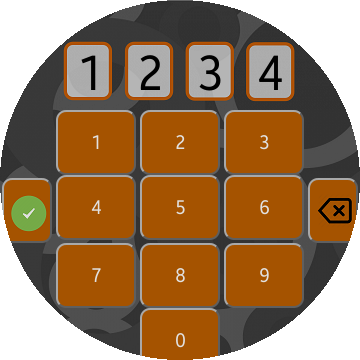
\includegraphics[width=3in]{images/login_screen.png} 
   \caption{login screen v1.0}
\end{figure}

After some testing and discussions it was decided that the feedback of the pressed numbers on the top of the screen were to small and thus some rethinking was needed to come up with a new design. An idea was to make four rotating disks that was inspired from securing a travel suitcases. 

\begin{figure}[H] %  figure placement: here, top, bottom, or page
   \centering
   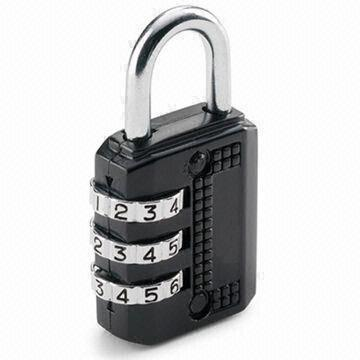
\includegraphics[width=3in]{images/lock.jpg} 
   \caption{lock}
\end{figure}

The advantage is that no buttons for the numbers were needed so the numbers could be place in the middle. In the middle they can be displayed in a larger font since more space is available due to the circular shape. However, the detection of swipe events were insufficient for rotating the disks and thus the idea for rotating disks was changed to improve the functionality. The positions of the numbers stayed the same, but instead of swiping an increase and decrease button was added above and below each number (see figure login\_screen\_2.png). 

\begin{figure}[H] %  figure placement: here, top, bottom, or page
   \centering
   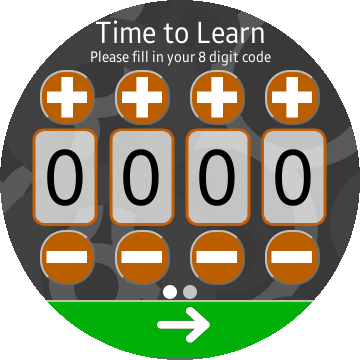
\includegraphics[width=3in]{images/login_screen_2.png} 
   \caption{login screen v2.0}
\end{figure}

To increase the safety of a user's account it was decided to use a code of eight digits and therefore a page indicator was placed below the decrease buttons to notify the user that the user should insert 4 digits two times. On the bottom of the screen a next button is placed to go to the next page for inserting the second 4 digits of the code or to confirm that the 8 digits were inserted.

\ok

\section{Main screen}

When a valid code is inserted, the main screen becomes visible. During the project, the main screen had had different layouts. All the decisions are sorted in different categories: time, words, background, buttons, information components, option lists, profile and effects.

\subsection{Time}

An important part of the app is displaying the time, since the app will be the first thing the user will see when the watch screen turns on. This importance was not clear at the beginning of the project, therefore the first design contained the time in a small black font. The size of the font was based on the hill that was displayed on the background. With the chosen font the time fitted in the hill in the middle to increase the readability (see figure version 1.png). \ok

\begin{figure}[H] %  figure placement: here, top, bottom, or page
   \centering
   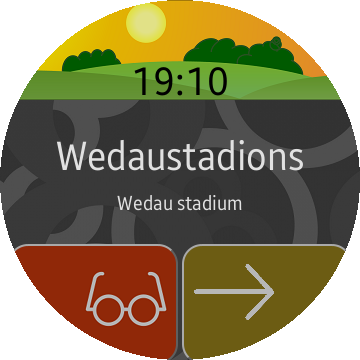
\includegraphics[width=3in]{images/version_1.png} 
   \caption{version 1}
\end{figure}

After the first discussion it was decided that the time should be displayed on 50\% of the screen since the app would be use for checking the time and for learning words (see figure version 2.png)\ml{References to figures are done like this Figure \ref{fig:version2}. Note that I've added the {\bf label} command to the figure environment. Please do all the references this way! Thanks!}. The time however was not readable enough and this was solved by changing the font color to white and by changing the background (see figure version 3.png). This new design worked \del{really} well and therefore this became the final design for the time. 

\begin{figure}[H] %  figure placement: here, top, bottom, or page
   \centering
   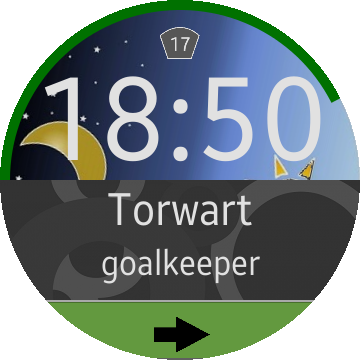
\includegraphics[width=3in]{images/version_3.png} 
   \caption{version 3}
\end{figure}

\subsection{Words}

The other important part of the app is showing the wordpairs, the word and the translation, the user wants to learn. Displaying wordpairs on a small circular screen was quite challenging which resulted in different designs for the watchface (see figure all possible versions.png). In the first design the wordpairs were placed in the middle of the screen (see figure version 1.png) with a white font.

 Due to the circular shape there is more space available in the middle of the screen and therefore the wordpairs can be in a larger font. The color white was chosen to have a maximum contrast with the background since the background mostly consists of dark colors. The words have a larger font than the translations to have a clear distinction between the two types and later on the smaller font was selected to make sure that there is enough space to display the translations. Since the translations are placed lower than the words, less space is available. 
When only 50\% of the screen was available for the wordpairs after the first discussion, the wordpairs were placed just below the middle where the space lost is minimal (see figure version 2.png).  

\begin{figure}[H] %  figure placement: here, top, bottom, or page
   \centering
   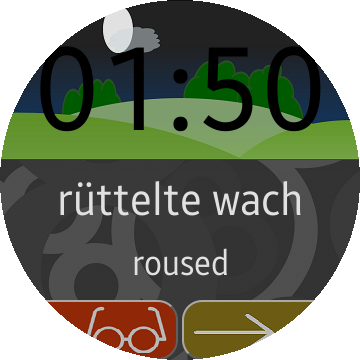
\includegraphics[width=3in]{images/version_2.png} 
   \caption{\chg{version 2}{The second version of the time display uses 50\% of the screen for showing the time.} \ml{Always have the caption of a figure together with the figure tell a story! }}
   \label{fig:version2}
\end{figure}

\subsection{Background}

The app consists of two parts, one for the time and one for the wordpairs. Both parts have different backgrounds. The background for the wordpairs was selected in the beginning of the project and did not change. The background consists of different dark grayish colors and with the white colored wordpairs the user should not have any problems reading the wordpairs.

At first the idea for the background of the time was that it should support the current time. Therefore four different backgrounds were designed for the morning, afternoon, evening and night (see figure first designs background.png). 

\begin{figure}[H] %  figure placement: here, top, bottom, or page
   \centering
   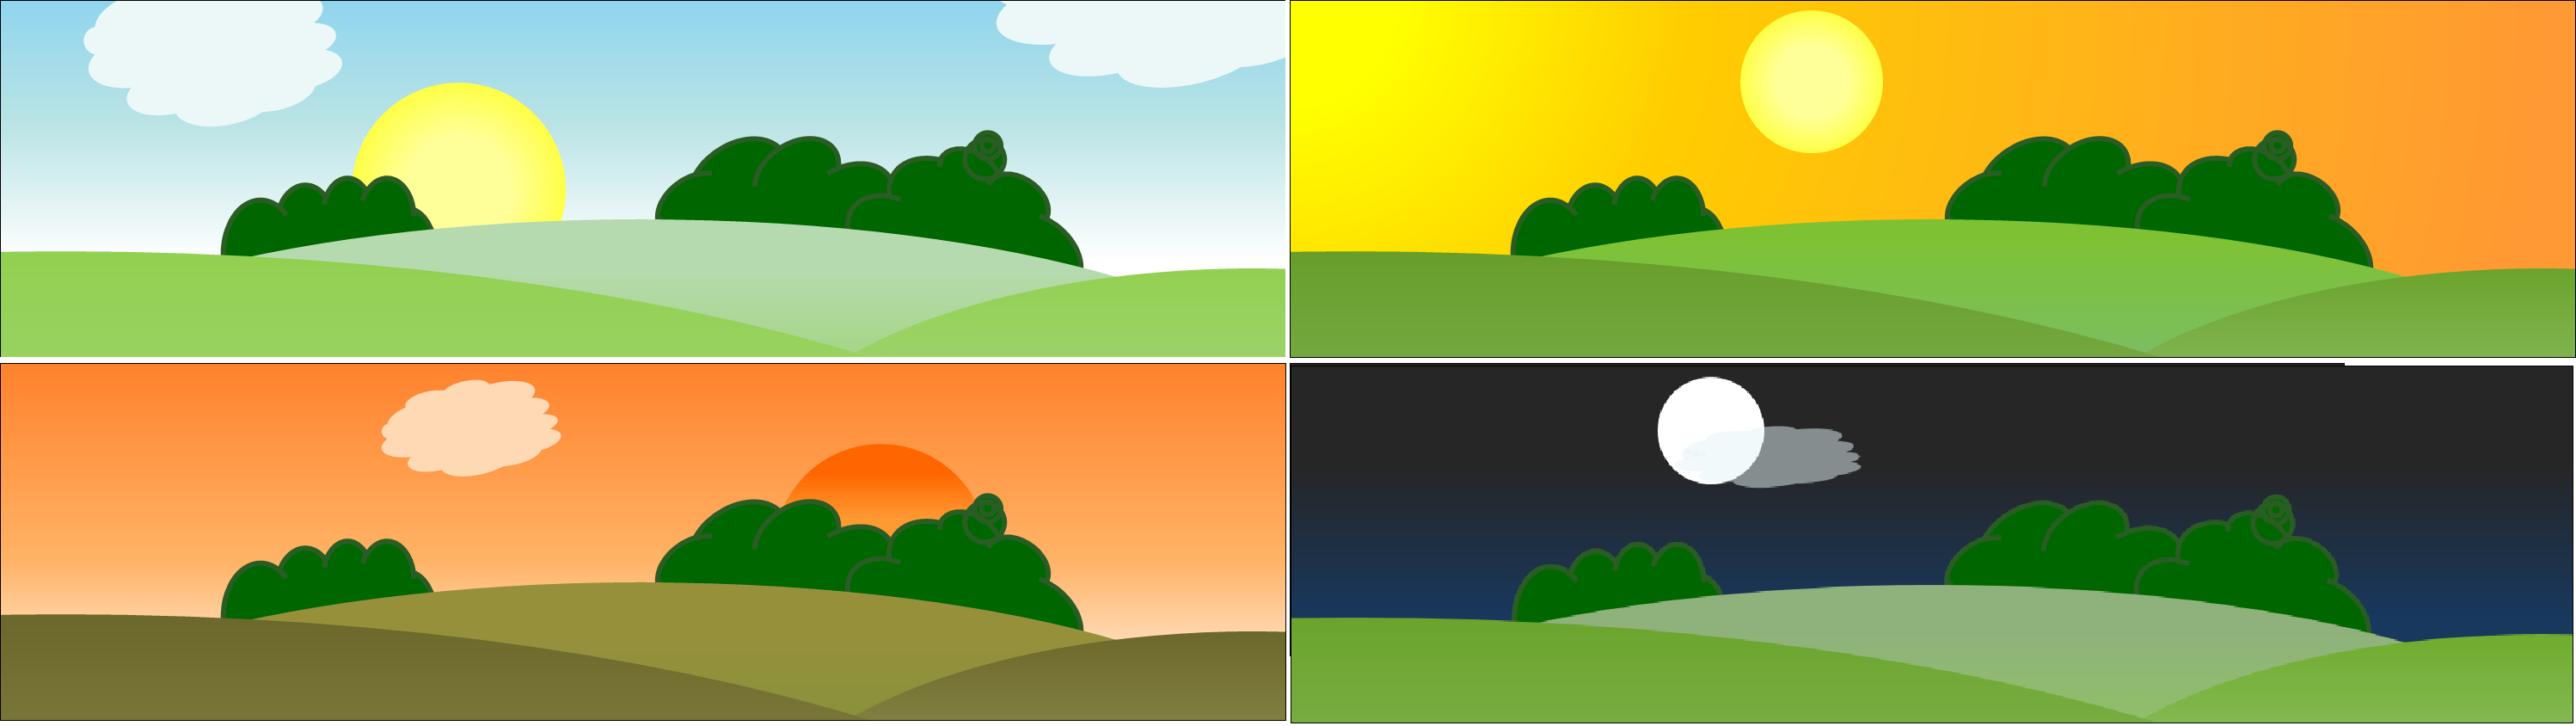
\includegraphics[width=3in]{images/first_designs_backgrounds.png} 
   \caption{first designs background}
\end{figure}

The space for the time then changed to 50\% of the screen and therefore the backgrounds were unusable because of the old dimensions of the images.
Instead of changing the images to the new dimensions this moment was used to think again about the background of the time. The different images for the different types of the day had to be saved on the watch. This storage issue was solved by using one image. The new background consisted of the sun, the moon and a transition between blue and black. This background rotated around it's center which makes it possible to support the current time with the positions of the sun and the moon (see figure day\_cycle\_2.png).

\begin{figure}[H] %  figure placement: here, top, bottom, or page
   \centering
   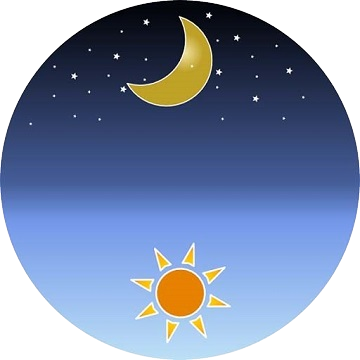
\includegraphics[width=3in]{images/day_cycle_2.png} 
   \caption{day cycle}
\end{figure}

Due to the rotation a sunset and sunrise could be seen on the watch. To emphasize the sunset and sunrise a landscape was added to make, for example, the sun appear from the horizon with a sunset. The used colors for the landscape were different from the colors in the rotating background and hence a new background with the sun and moon was designed to match the landscape (see figure version 5.png). The landscape worked really well with the rotating background and therefore two other landscapes were designed from which the user can choose (see figure designs landscape.png).

\begin{figure}[H] %  figure placement: here, top, bottom, or page
   \centering
   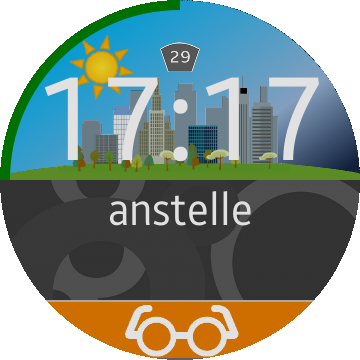
\includegraphics[width=3in]{images/version_5.png} 
   \caption{version 5}
\end{figure}

\begin{figure}[H] %  figure placement: here, top, bottom, or page
   \centering
   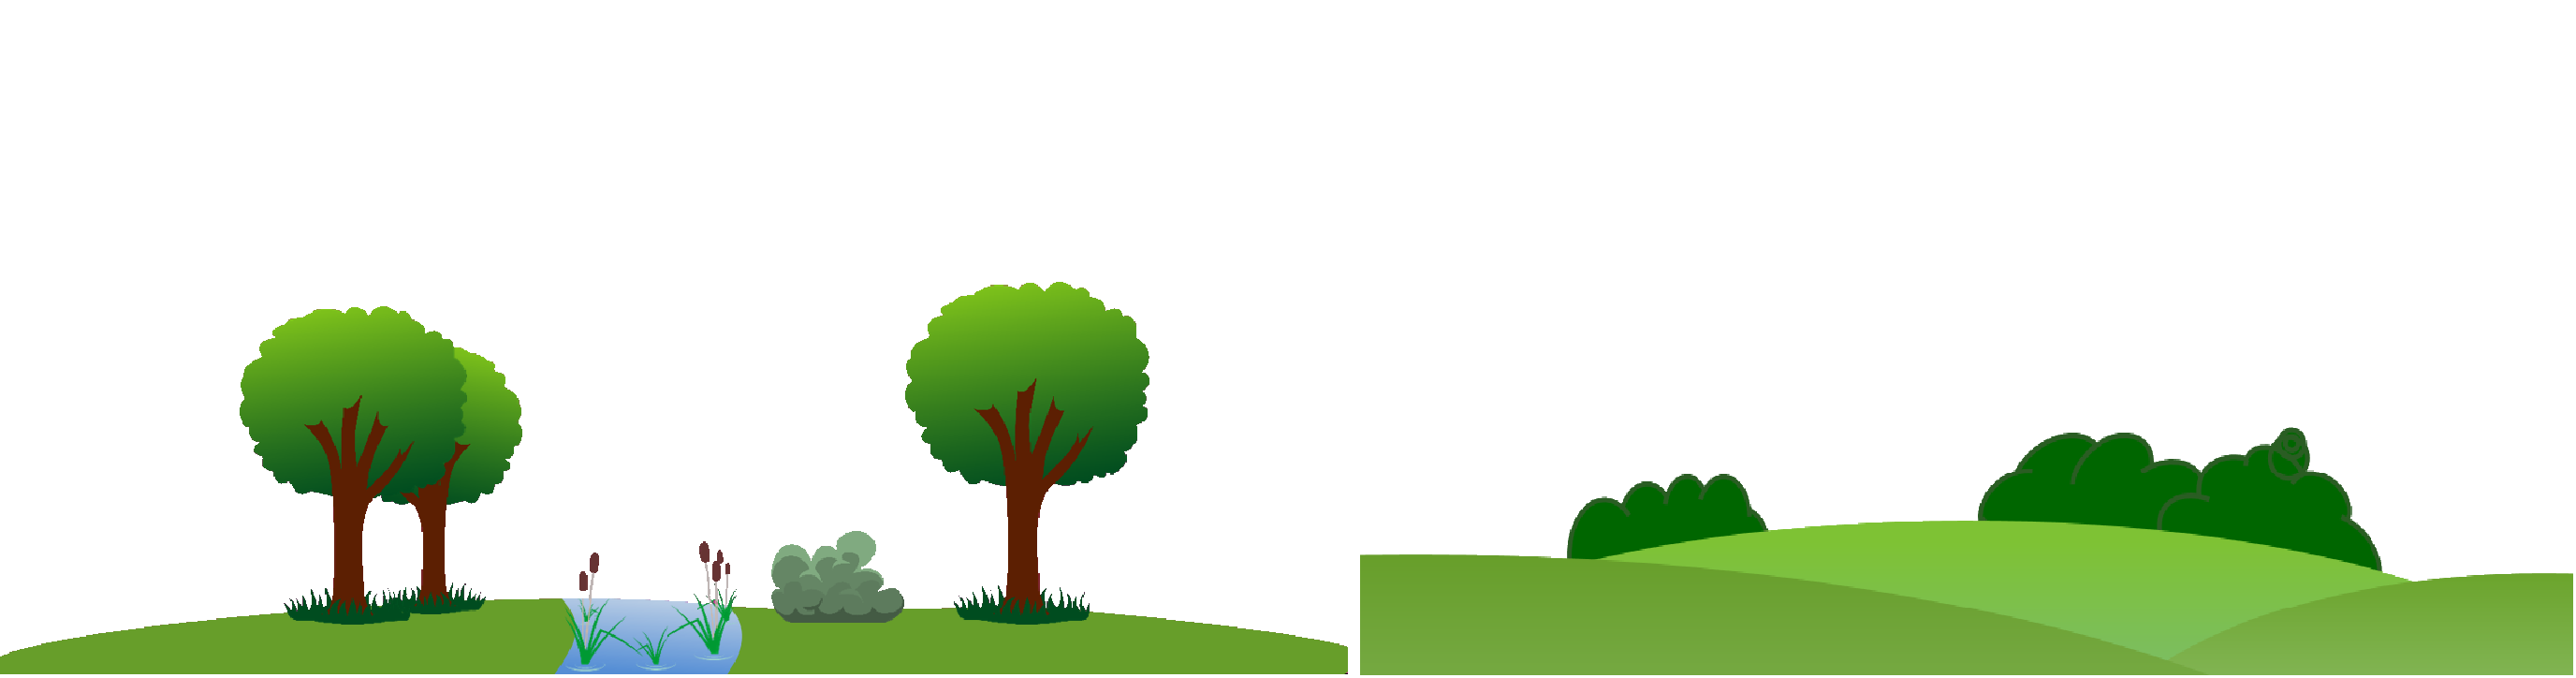
\includegraphics[width=3in]{images/designs_landscapes.png} 
   \caption{landscapes}
\end{figure}


\subsection{Buttons}

As mentioned before swipe detection was insufficient so it was decided that the app should only use touch events. To navigate through the app with only touch events it seemed logical to use buttons. With the time on top of the screen and the wordpairs in the middle there was unused space in the bottom for the buttons. In the first design the user should be able to reveal the translation of the shown word or to go to the next wordpair. This resulted in two buttons, a red one with glasses on it and one with an arrow to the right (see figure version 1.png). Glasses were chosen for revealing because it could refer to looking something up and that matches with revealing the translation. Since the app is displayed on a small screen, the buttons should not be to small and thus almost all the available space in the bottom was used for the buttons to ensure that there was enough space for the user to press a button. Different tests showed that the buttons could be made smaller. This was a favorable conclusion since after testing it was decided that only 50\% will be used for the wordpairs (see figure version 2.png). The design of the buttons was not really pleasing and needed some rethinking. The first modification was erasing the reveal button. Instead of the button the user could touch the word to reveal the translation. The 'next' button was widened so it covered the bottom of the screen (see figure version 3.png). 
During development more options were implemented and therefore a new button was made next to the 'next' button. The settings button gave access to these options (see figure version 4.png). The curves on the buttons as can be seen in the first design were replaced with right angles to create a modern feeling.
The app was tested and more attention was paid to improve the order in which the wordpairs are shown. This process should become smarter by use a knowledge estimator that would estimate what the next word should be to maximize the learning process. This estimation could only be made when the server could receive feedback of every single word. It is therefore necessary that the user should give feedback after every word. The design of the app was adapted to this new idea by changing the 'next' button to a 'reveal' button (see figure version 5.png). When the user pressed this button the translation appeared and the 'reveal' button changed in three different buttons: a 'wrong' button, a 'menu' button and a 'right' button (see figure version 5 reveal.png). This new design forced the user to give feedback after every word. This feedback could be used to optimize the order of the words. The first design of the buttons were a cross and a checkmark to let the user know what to press when a word was not know or was known. Later on a book and a graduation cap were used for the same purpose but the feedback to the user would be less harsh with the new design (see figure version 6 reveal.png).

\begin{figure}[H] %  figure placement: here, top, bottom, or page
   \centering
   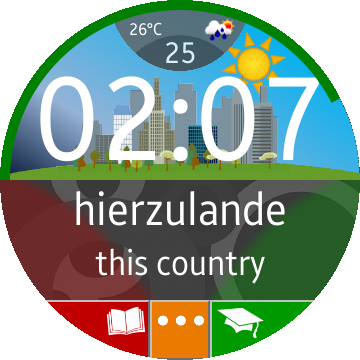
\includegraphics[width=3in]{images/version_6_reveal.png} 
   \caption{version 6 on revealing}
\end{figure}

\subsection{Information components}

Besides the time the app also shows the date. The date was added later when the design of the time was completed. In the first place the date had his own small icon on top of the screen (see figure version 3.png). This icon was partly covered by a Tizen icon for the swipe down menu. Therefore the icon for the date was moved downwards near the time (see figure version 5.png).
During a discussion it was mentioned that it would be nice to be able to see the temperature and the weather type on the watchface. After some research a free api* was found that could provide the app with this information. In the beginning of the implementation the temperature was placed to the left of the date and the weather type was placed to the right of the date. This was barely readable and it did not fit in the realized design hence a new icon was designed that contained the date, temperature, weather type and an open area in the middle for the Tizen icon for the swipe down menu (see figure version 6.png).

\begin{figure}[H] %  figure placement: here, top, bottom, or page
   \centering
   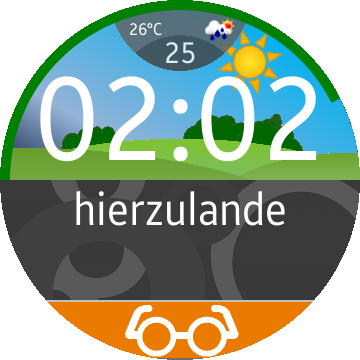
\includegraphics[width=3in]{images/version_6.png} 
   \caption{version 6}
\end{figure}

\subsection{Option lists}

The app has access to two different option lists: the settings which can be reached by double tapping on the time and the menu that can be reached by tapping in the middle of the translation. This was different in one of the first designs.
When the app was able to show the words with the translation, the user should have an option to tell the app that a word had a wrong translation or that a word was learned and thus in both cases it should not reappear again. Due to the small screen it was not convenient to add more buttons for each of these options to the watchface and therefore the idea came to make a menu with these extra options. Besides these options the user should be able to reverse the order in which the wordpairs were asked (when the words were displayed from German to English, the words would be displayed from English to German after the button was pressed), to insert the number of words that the user wanted to learn and to log out of the app. All these options were reachable for the user by a 'menu' button in the bottom. The 'next' button was replaced by two buttons, the 'menu' and the 'next' button (see figure version 4.png). 

\begin{figure}[H] %  figure placement: here, top, bottom, or page
   \centering
   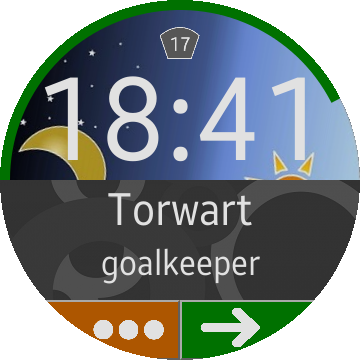
\includegraphics[width=3in]{images/version_4.png} 
   \caption{version 4}
\end{figure}

\begin{figure}[H] %  figure placement: here, top, bottom, or page
   \centering
   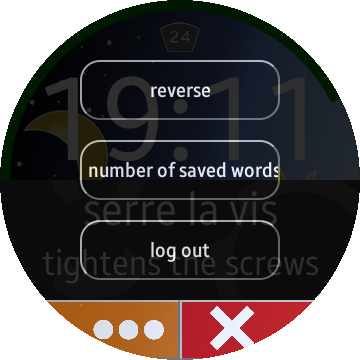
\includegraphics[width=3in]{images/version_4_settings_1.png} 
   \caption{version 4 settings}
\end{figure}

When the 'menu' button was clicked a menu would appear with the 'trash' button and the 'I learned it' button.  In the bottom the user could close the app or open the settings (see figure version 4 menu 1.png). By pressing the 'settings' button the user would open the settings page with the buttons for reverse, number of words and log out (see figure version 4 settings 1.png).
After some discussions the overall opinion was that the 'menu' button should not be this large on the watchface since the menu would give complementary options which were not part of the main function of the app. Therefore the button should not cover half of the bottom and a solution was to split the menu and the settings to two different pages that the user could reach independently. The user could reach the menu by tapping in the middle of the translation (see figure version 5 reveal.png) and the settings could be reach by double tapping on the time since this space was hardly used. The double tap was necessary because tapping the time would change the background.
The menu and the settings both had a black transparent background for a long time. This was inspired from the transparent and blurred swipe down menu from a well-known OS. Unfortunately the blur effect was not a success, but the transparency remained.

\begin{figure}[H] %  figure placement: here, top, bottom, or page
   \centering
   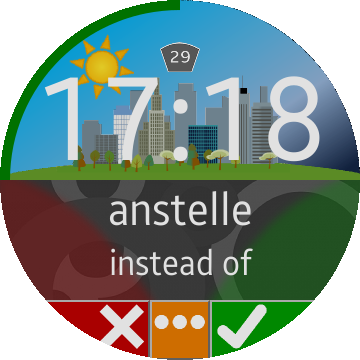
\includegraphics[width=3in]{images/version_5_reveal.png} 
   \caption{version 5 reveal}
\end{figure}

During testing the text in the buttons were hard to read and the buttons of the main page were visible through the buttons on the bottom. Therefore it was decided that the menu and the settings page should have a background. For the background the same image was used as the background of the wordpairs to preserver the unity of the design.
A lot of translations depends on the context of the word. Hence the user should be able to see the context of the word and this option was added to the menu page (see figure version 6 menu.png). 

\begin{figure}[H] %  figure placement: here, top, bottom, or page
   \centering
   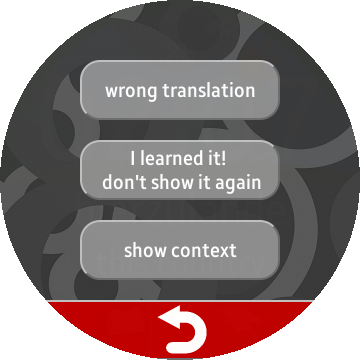
\includegraphics[width=3in]{images/version_6_menu.png} 
   \caption{version 6 menu}
\end{figure}

Later on  the idea was abandoned of letting the user choose how many words the user wants to learn and instead came the 'profile' button as the latest addition to the settings page (see figure version 6 settings.png).

\begin{figure}[H] %  figure placement: here, top, bottom, or page
   \centering
   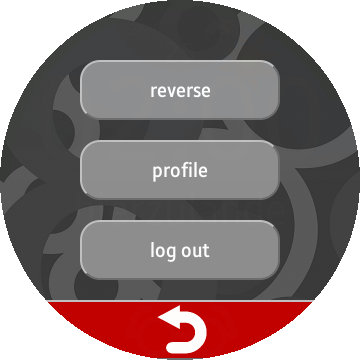
\includegraphics[width=3in]{images/version_6_settings.png} 
   \caption{version 6 settings}
\end{figure}

\subsection{Profile}

One of the latest addition to the app was the implementation of a profile page where the user could see the four medals that could be earned by using the app (see figure version 6 profile.png). The four categories are: words learned, total time, longest session and longest streak. 
This page was inspired from a presentation where gamification was mentioned. The idea was that when users could earn medals, users would be more willing to use the app. 
When the user presses the 'I learned it' button, the number of 'words learned' will increase and after 10 new learned words, a popup will appear with a motivating message to continue. 
The total time the user used the app is also registered. When this time is the same as one of the pre-determined minutes a popup appears (see figure version 6 popup.png).
With longest session the time is measured that the user uses the app  continuously and with the longest streak the number of days is registered in which the app is used daily. One day of not using the app resets the longest streak.

\begin{figure}[H] %  figure placement: here, top, bottom, or page
   \centering
   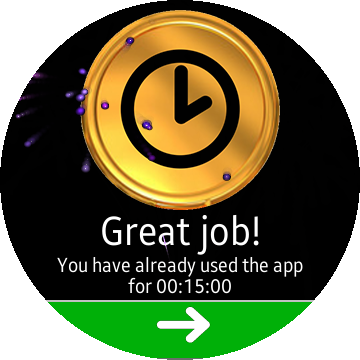
\includegraphics[width=3in]{images/version_6_popup.png} 
   \caption{version 6 popup}
\end{figure}

\subsection{Effects}

To improve the experience of the app some effects were added: to give feedback after a button was pressed, to give information (why an option was not available or why a medal was earned) or to beautify a popup.
Because of the small screen the user could think the wrong button was pressed and therefore the user should get feedback about which button was pressed. The most important buttons in the app are the buttons used for indicating whether a word was known or not. When one of these buttons is pressed a green or red image appears depending on if right or wrong is pressed. This image stays on the display for a few milliseconds before it fades out.
In the app several popups are added to give the user feedback when an option is not available. The design of the popup is based on the first design of the option lists. The popup has a black transparent background with white text on it. The popup could appear when: there is no connection with the internet, when a wrong code is inserted, when the user has too few words, when there are too few words left on the watch or when a user earned a new medal.
The popup that appears when a new medal is earned is beatified by some fireworks.

\chapter {The Implementation}
In this part the implementation choices are described. In this project writing the code was one of the biggest challenges. The code has been changed a lot during the process. One of the reasons was to increase readability, but also because of design changes and new features which had to be implemented. The code is written in JavaScript in combination with HTML 5, this means it is web-based application. The code is build with a framework called requirejs, this makes it possible to have multiple files (modules) in javascript, this to increase readability and structure. In the following sections, we will zoom in some interesting and important decisions and choices related to the implementation.

\section{Flash card algorithm}
For presenting the words we used a certain algorithm. This algorithm will make sure users will learn faster and it's based on the flashcard method. The algorithm works in such a way that words which are answered wrongly will be faster repeated than words which were answered correctly. As explained in the design the user can indicate whether he had the answer wrong or right in his head. If the user had it wrong the word will be repeated after five more words, when the user had it right in his head the word will be repeated depending on the number of times the user had it correct. The word will be $timesCorrect * 5$ positions moved in case the user the had it right in his head. In figure 4.1 this process is shown. 

\begin{figure}[H] %  figure placement: here, top, bottom, or page
   \centering
   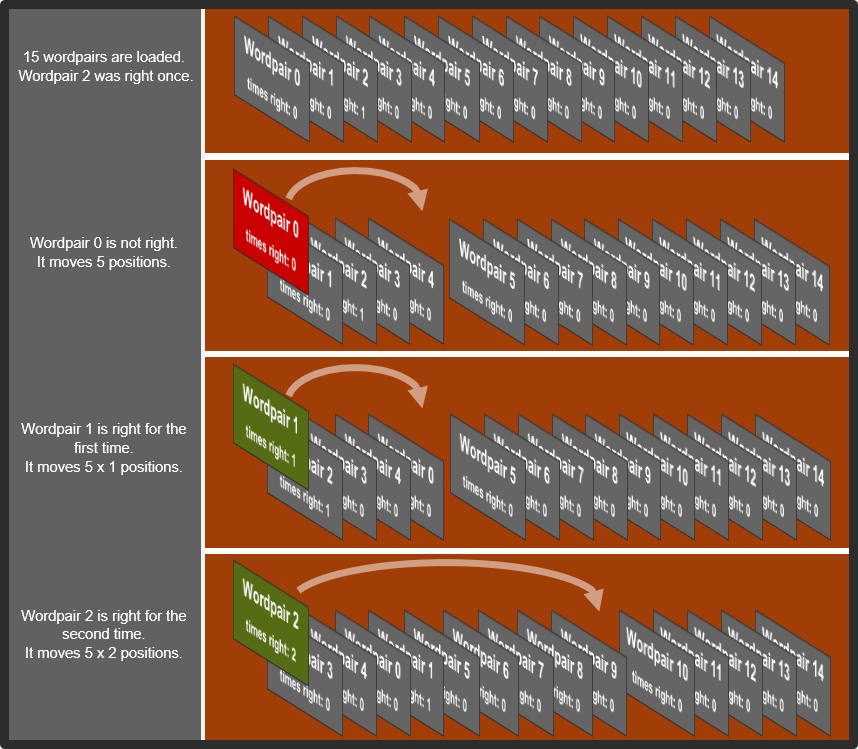
\includegraphics[width=5in]{images/flashcard_method.png} 
   \caption{Flashcard simulation}
\end{figure}

In listing 1 the code involved is shown, every time the users taps wrong or right the function $updateWordPair$ is called, if the user had it right the number of times correct will be increased. After that the current word will be moved in the array. This happens by first adding the word some positions further and then deleting the current word (i.e., deleting element zero in the array). If the user taps wrong the current progression will be reset (i.e, timesCorrect becomes zero again), and the word will be moved five positions to the right (see figure 4.1). This means the word will be repeated reasonably fast. Because the first element of the array is always shown on the screen, the next word will be drawn on the screen, since the previous first element is deleted. In $userData.js$ everything related to the user is implemented, so this is the place where words can be found. A wordPair is characterized with the following attributes: word, translation, id, context and number of times correct. Getting the word pairs from the server is explained in the next section.

\newpage

\lstinputlisting[language=JavaScript, firstline=49, lastline=59, caption=flashcard implemenation in userData.js]{source_code/userData.js}

\section{Getting new words from the server}
In the module session.js the words are fetched from the server. This session is created in the main.js. The code which login gives (either entered by the user or loaded from the userData) will be used in session.js to get the words for the user. The session can get new words with this unique code. The code is generated once a new account is created and can be found in the account when logged in the browser. The code contains eight digits. When a session is created, the first thing to look at are there currently any words on the watch. If there any words on the watch we can set the status to `succes', in case there are no words on the watch yet: the watch has to communicate with the server and get the words with the endpoint `bookmarks\_to\_study'. This endpoint will return the words which are currently the most important to study for that particular user. In the implementation we made the choice to get fifty words in case the user has no internet for longer periods of time. The session can return different states: if the words are successfully fetched from the server the state will be `succes' as described earlier, if the code is invalid the state will be 'wrong session number', in case of no internet connection the state will be 'no connection'. There is one exception, but this will not happen very often this is when there are too few words in the account of the user. One of these states will be returned to the main module and the main module will give this state through to the login module, in the login the user can then be informed by a popup that will inform the user about a specific situation. If the state was `succes' the user will get in the main screen where the words are presented. The login module is not the only place where the watch tries to get new words, it also happens when the user is already logged in and a screen on event occurred (i.e., user makes arm twist to look at time). The new words will then be added to the current wordlist on a screen off event (i.e., user makes again a arm twist to indicate he is not looking anymore), adding words at this point is to prevent any conflicts: adding words to a list which the user is currently doing stuff with. New words will only be added if the list is smaller than fifty words. The list can become smaller if the user has marked a couple of words as `learned it' or as `wrong translation'. When writing the code the initial preference was to get words and add them at the same time on a screen off event, since the user won't be using the application at that moment and it would really feel as everything happens in the background. Unfortunately this didn't work the watch gets in a sort of sleep modus and won't be able to communicate with server anymore. The GET request wasn't executed so it was impossible to do this on a screen off event. When the watch tries to get new words from the server, this happens asynchronously to prevent the watch from getting slow. Implementing this asynchronously was huge in the eind, because the user is able to get a lot of words in his account (e.g., some user had already 10000 words) the endpoint will be really slow, since the list of words is not already sorted on importance on the server server side. In the first implementation when it was implemented synchronously, therefore the user could have some delay before being able to interact with the watch. It was first implemented in this way to prevent conflicts, user cannot do something with a list while words are being added. This is now solved by getting the new wordPairs on a screen on (see listing 2) and add them later on a screen off (see listing 3).

\lstinputlisting[language=JavaScript, firstline=48, lastline=62, caption=getting new wordPairs in session.js]{source_code/session.js}

\lstinputlisting[language=JavaScript, firstline=32, lastline=35, caption=adding new words to wordPair in userData.js]{source_code/userData.js}



\section{Usage Tracking}

\subsection{Events}
Events are implemented to give the knowledge estimator information which can be used to analyse the knowledge of the user. The knowledge estimator is on the server side implemented. This means we had to decide at what point we should send the events. Because the knowledge estimator decided what the next word is going to be for the user, the events should be send when the user taps wrong or right. This is the moment the user will be presented with a new word. The knowledge estimator can receive the following events: reveal, right, wrong, wrong translation, I learned it, showContext, screenOn and screenOff. 

\subsection{Clicktracking}
The clicktracker is designed for research purposes. It's purpose is to track where the user clicks/taps, so the coordinates are saved. Not only the click position is saved, also the click type (e.g., user taps on reveal). For some function this can be really interesting like the right button; the user can tap on the button itself or on the green space above the button. Both actions result in the same thing. In the future we could change the design based on these results to give the user a better experience. To conclude the clicktracker is nothing functional, it is purely for research purposes. 

\section{Changing the watchface and sending and saving}
Sending and saving the clicks and events was a big challenge in this project. This is the result of the user being able to change the watch face at every moment, which will result in losing data. Because the user is able to go a different watch face at any moment clicks and events should be saved to the storage of the watch immediately. We do this by saving it to the local storage. This is is implemented in the same way as saving to the local storage in a web browser. The application is web-based using JavaScript and HTML, which was already explained earlier on. A click and event are immediately pushed to the storage after they occurred. The clicks in the storage are send on a screen on event asynchronously, so it won't influence the speed of the application and it happens in the background. When the clicks are successfully send to the server, the server will return `OK', if the watch then receives this message the clicks in the storage can be freed, they are now at the server. The events in the storage are send on `right' and `wrong' as earlier on explained to inform the knowledge estimator. Just as with the clicks the events are deleted from the storage if they successfully have been arrived on the server side. Losing data with changing the watch face not only happens with clicks and events, it also happens when the user reverses the way the words are asked (e.g., English - Dutch to Dutch - English) and with changing the background. The login code is being saved the first time and used for automatic login after a watch face change. 

\section{Drawing the userinterface}
The userinterface is drawn every second on the screen, this happens in gui.js in the draw function which is public (shown in listing 4). The main module has an function which calls this function in gui every second (shown in listing 5). The screen is thus updated every second. Time and profile are also being refreshed in the draw function, in the future it would be nice to have these in a different function to make sure draw only draws stuff. 

\lstinputlisting[language=JavaScript, firstline=153, lastline=163, caption=draw function in gui.js]{source_code/gui.js}

\lstinputlisting[language=JavaScript, firstline=11, lastline=14, caption=main class]{source_code/main.js}

\chapter{Usage study}
After the implementation the app was ready to enter the test phase. The results of the test period should give answers to the following two questions: is the app used during short intervals (this would indicate that the users used the app for micro-learning) and is the app designed properly (e.g., are all the option found during the test period).

The test period consisted of four parts:
\begin{enumerate}
\item All participant started with making an account on Zeeguu in which they saved several words they wanted to learn.
\item The participant received the smartwatch with the app as a watchface and basic instructions about how to use the app.
\item The participant used the app for four days in a row.
\item After four days the participants handed in the smartwatch and they filled in a questionnaire about the test period and how they experienced the app.
\end{enumerate}

During the test period the smartwatch kept track of the usage by using telemetry. All the buttons and touch areas for the existing options had different events attached to it so when a button or area was pressed, an event would be made and sent to the server. The events and their definitions are shown in table 5.1. 

\begin{table}[H]
\centering
\caption{Events}
\begin{tabular}{| l | p{10cm} |} 
\hline
\textbf{Type} & \textbf{Definition} \\ \hline 
screenOn & When the screen lightens up. \\ \hline
reveal & When the user wants to see the translation and presses the `reveal' button or area. \\ \hline
right & When the user knows the translation and presses the `right' button or area. \\ \hline
wrong & When the user does not know the translation and presses the `wrong' or area. \\ \hline
wrongTranslation & When the user thinks the translation is incorrect and presses the `wrong translation' button in them menu. \\ \hline
learnedIt & When the user thinks the word is learned and presses the `I learned it' button in the menu. \\ \hline
showContext & When the user wants to see the context of the word and presses the `show context' button in the menu. \\ \hline
reverse & When the user wants to learn the other way around and presses the `reverse' button in settings. \\ \hline
screenOff & When the screen turns off. \\ \hline
\end{tabular}
\end{table}

Besides the type of buttons or areas the position of the tap was also sent to the server. With this extra data a heat map could be made that would reveal the most used positions for the different options. However an object was sent to the server while the server expected a string due to miscommunication. 

\section{Usage results}
After all the participants finished their test period all the events per user were collected from the server and analyzed. For answering the research questions and for giving a clear overview about how the app was used during the test period, the following diagrams were made per user:
\begin{itemize}
\item \textbf{A circle diagram about the overall usage of the smartwatch in seconds (see fig. 5.1 and 5.2).} The diagram about the overall usage was created by collecting all the time intervals between a `screenOn' and a `screenOff' event. This data was then sorted into five different intervals:
\begin{itemize}
\item time $\leq$ 2
\item 2 $<$ time $\leq$ 5
\item 5 $<$ time $\leq$ 15
\item 15 $<$ time $\leq$ 60
\item time $>$ 60
\end{itemize}
The first interval was chosen, because checking the time or other arm movements would not take more than two seconds. When the duration is longer than two seconds the user probably does more than only checking the time. 
The user could check the time, but because a word is shown too, the user might reveal that word by pressing `reveal' and then the user might also give feedback by pressing `right' or `wrong'. These actions for one word would take not more than five seconds. Summarized, these could be learning sessions that were not intended to be a learning session. Then comes the intended learning sessions but for a really short time and the sessions that took a bit longer. As mentioned before the learning app will probably only be used for short sessions and thus sessions longer that one minute will probably hardly occur.
\item \textbf{A circle diagram about the duration of the learning sessions on the app in seconds (see fig. 5.3 and 5.4).} The duration of the learning sessions were found by using an algorithm (see listing 6). This algorithm first sorted out all the `screenOn' events that were immediately followed by a `ScreenOff' event. A user that used the app for learning and not for checking the time would use at least one option the app provides for learning new words before the screen would turn off. Therefore the combinations of a `screenOn' and `screenOff' events were seen as not learning sessions and these pairs were erased from the list of events. 
In the remaining events the time was measured between a `screenOn' and a `screenOff' event and afterwards the data was sorted into four intervals: 
\begin{itemize}
\item time $\leq$ 5
\item 5 $<$ time $\leq$ 15
\item15 $<$ time $\leq$ 60
\item time $>$ 60
\end{itemize}
The app will presumably be used for micro learning. Therefore the number of sessions will probably decrease exponentially when the duration increases. This is the reason why the length of the intervals increases faster than a linear growth.
\item \textbf{A bar chart about the number of times a user pressed `right' and `wrong' (see fig. 5.5 and 5.6).} 
For each day the app was used the number of `right' and `wrong' events were counted and plotted in a bar chart. 
\item \textbf{A table with the average reaction time between a `reveal' and a `right' or `wrong' and the time the app was used.} The reaction time is the time it took the user to press `right' or `wrong' after `reveal' was pressed. The average was calculated for each single day and for the whole period of four days. Besides the average time the total time is mentioned too. This indicates for how long the user used the app during the four days of testing.
\end{itemize}

\begin{figure}[H]%
    \centering
    \subfloat[Testperson 1]{{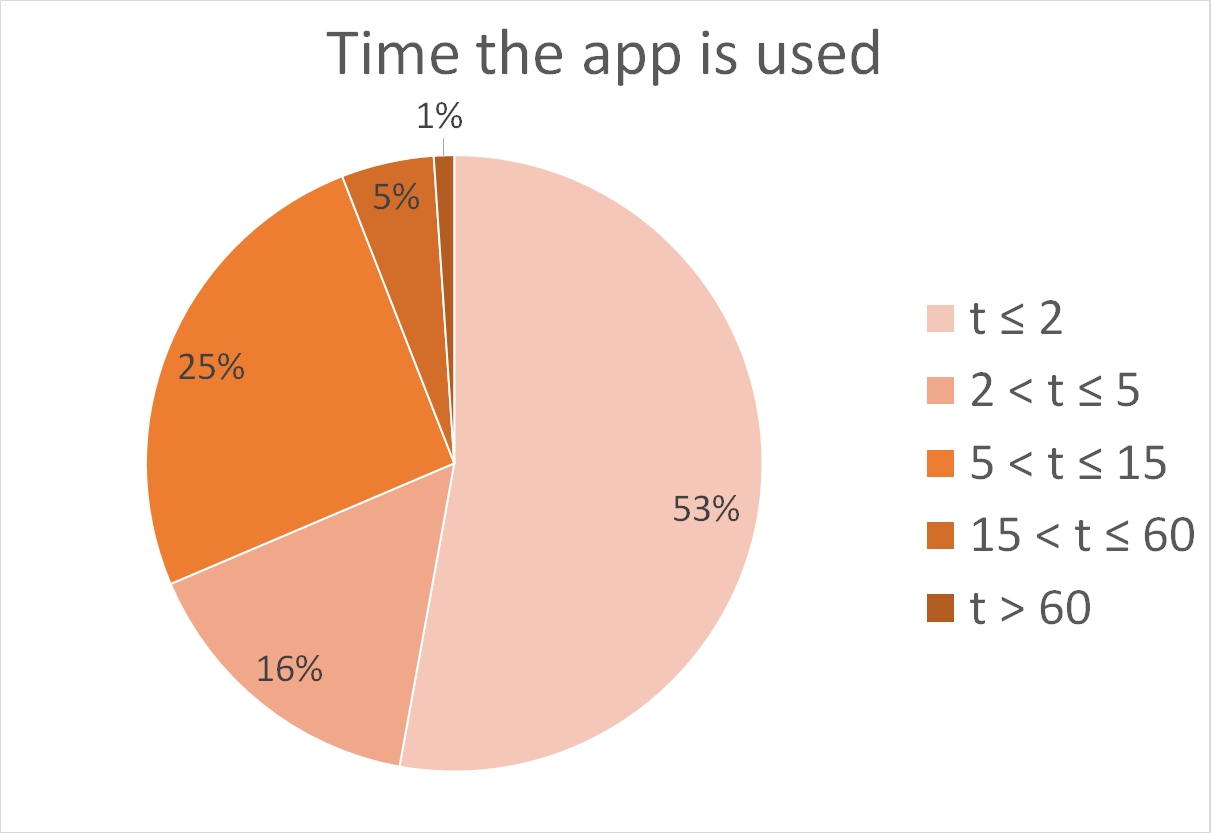
\includegraphics[width=2.6in]{usage_results/1_usage.png} }}%
    \qquad
    \subfloat[Testperson 2]{{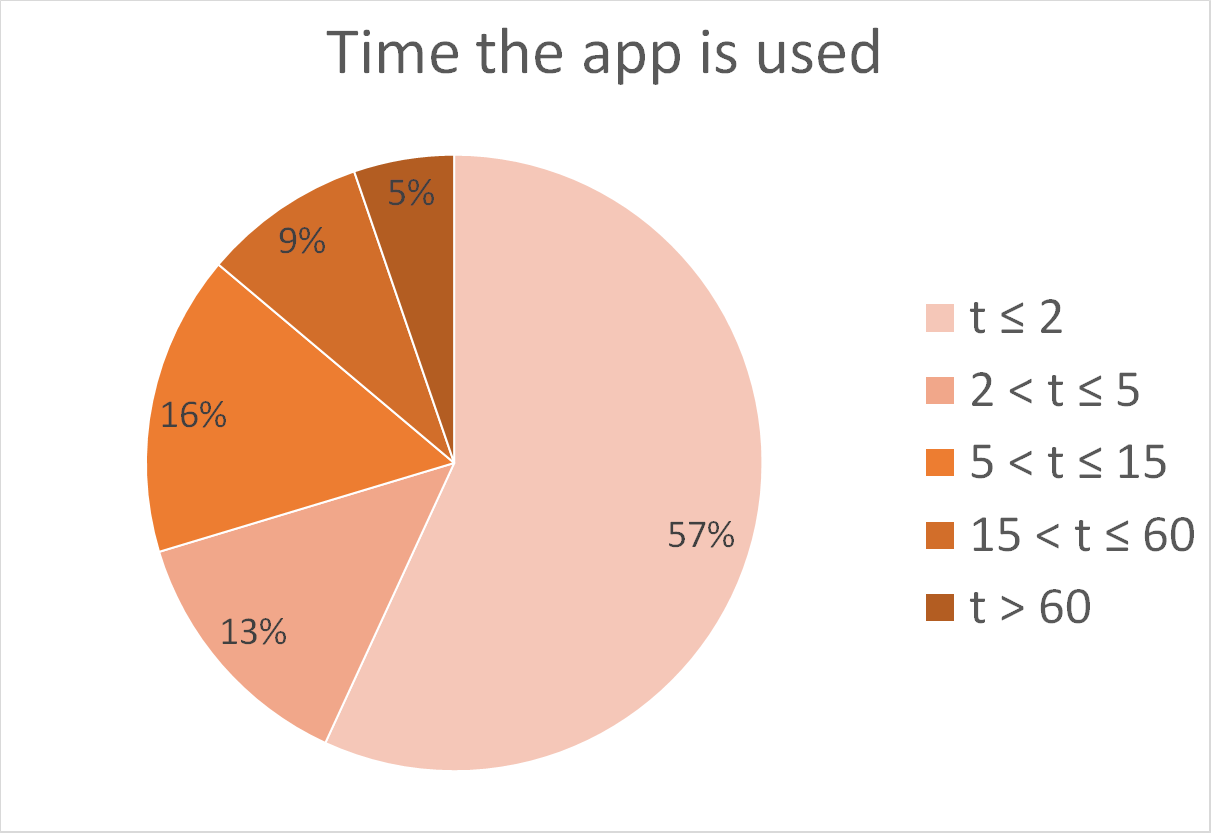
\includegraphics[width=2.6in]{usage_results/2_usage.png} }}%
    \caption{General usage testpersons 1 and 2}%
    \label{fig:example}%
\end{figure}

\begin{figure}[H]%
    \centering
    \subfloat[Testperson 3]{{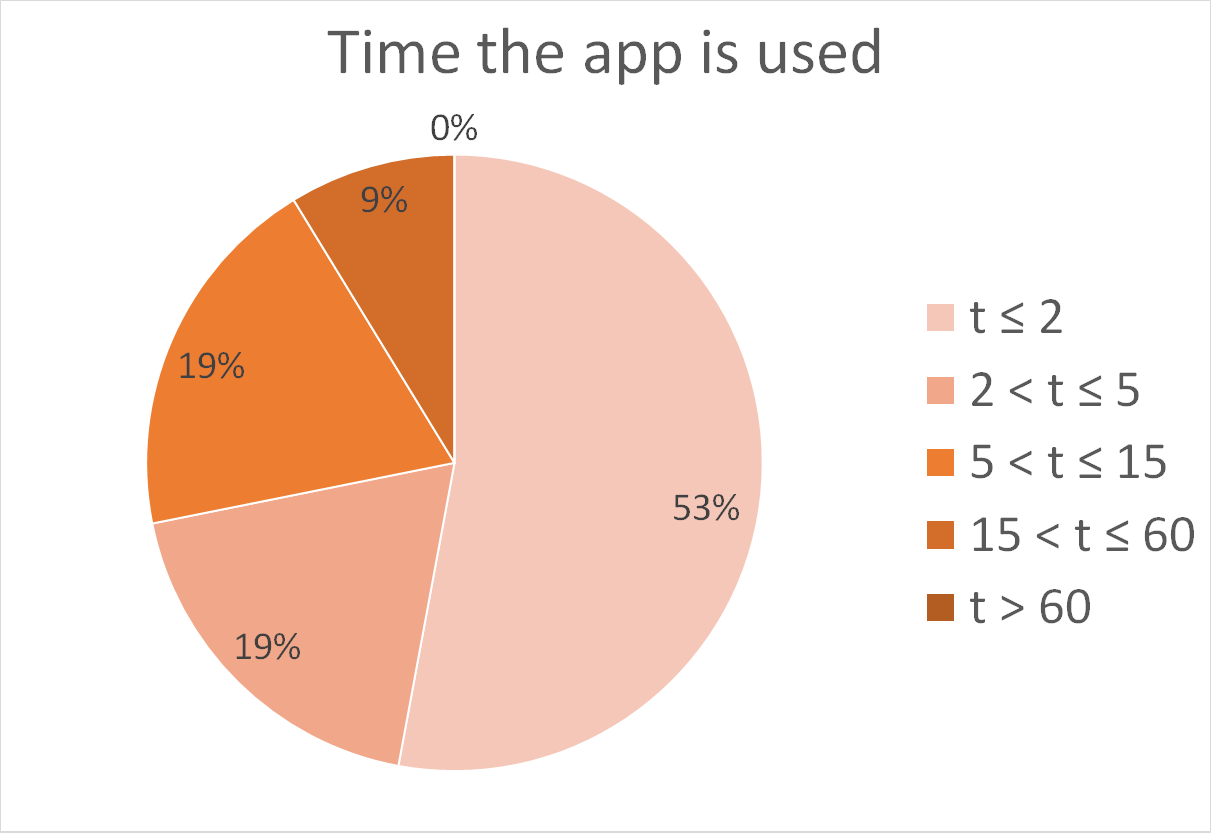
\includegraphics[width=2.6in]{usage_results/3_usage.png} }}%
    \qquad
    \subfloat[Testperson 4]{{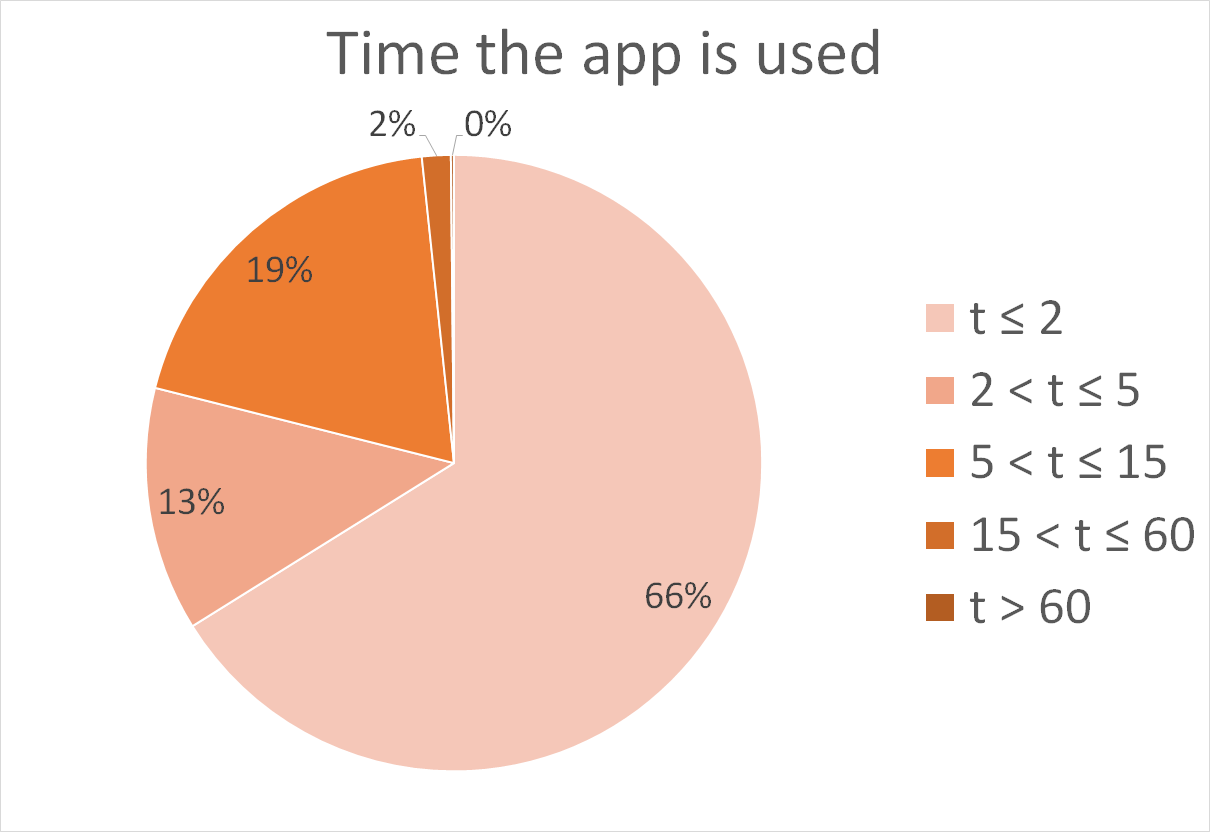
\includegraphics[width=2.6in]{usage_results/4_usage.png} }}%
    \caption{General usage testpersons 3 and 4}%
    \label{fig:example}%
\end{figure}

\begin{figure}[H]%
    \centering
    \subfloat[Testperson 1]{{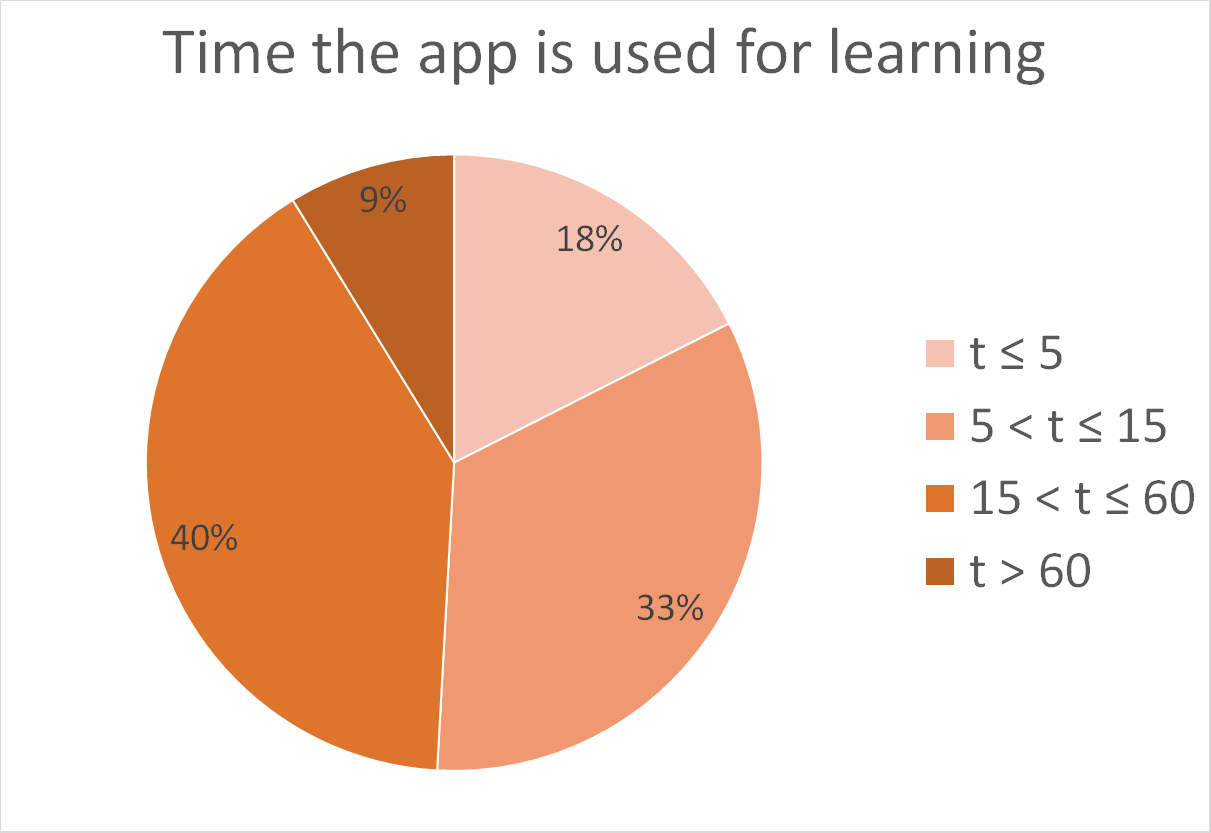
\includegraphics[width=2.6in]{usage_results/1_usage_learning.png} }}%
    \qquad
    \subfloat[Testperson 2]{{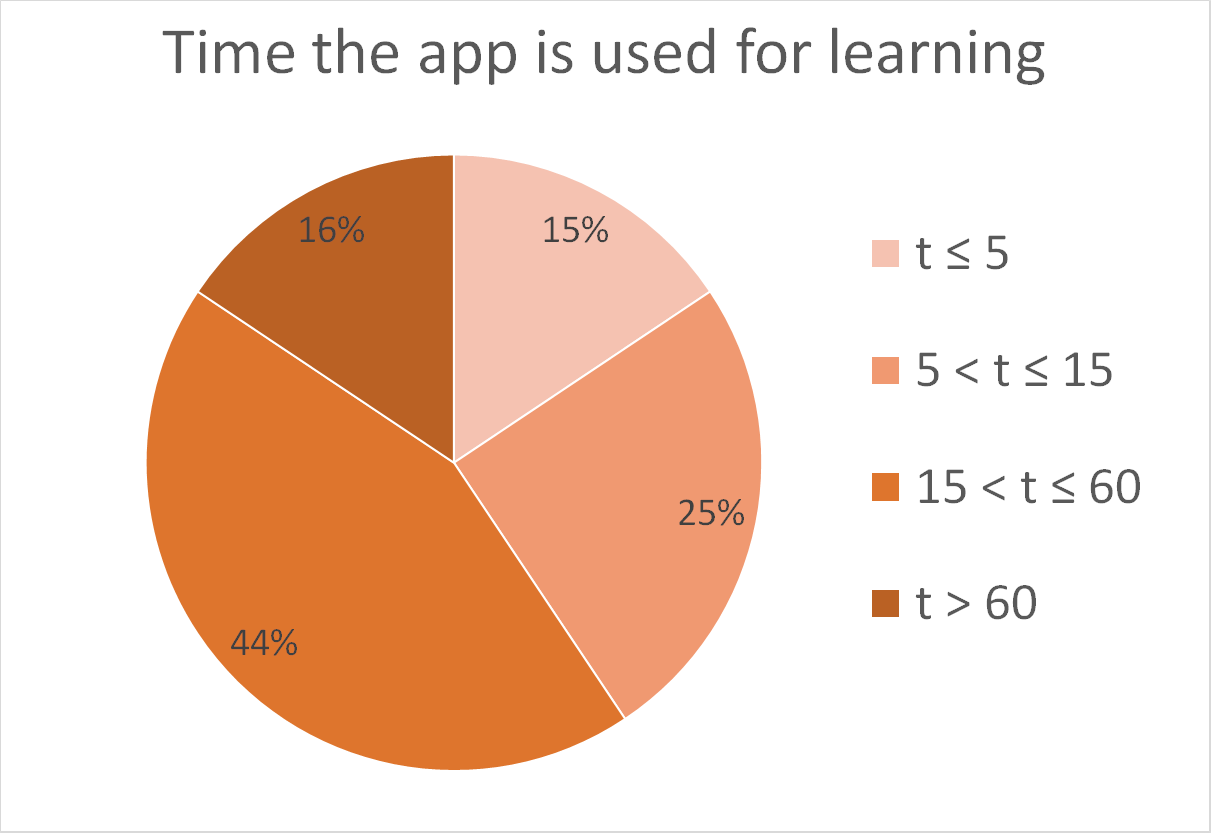
\includegraphics[width=2.6in]{usage_results/2_usage_learning.png} }}%
    \caption{Learning sessions time testpersons 1 and 2}%
    \label{fig:example}%
\end{figure}

\begin{figure}[H]%
    \centering
    \subfloat[Testperson 3]{{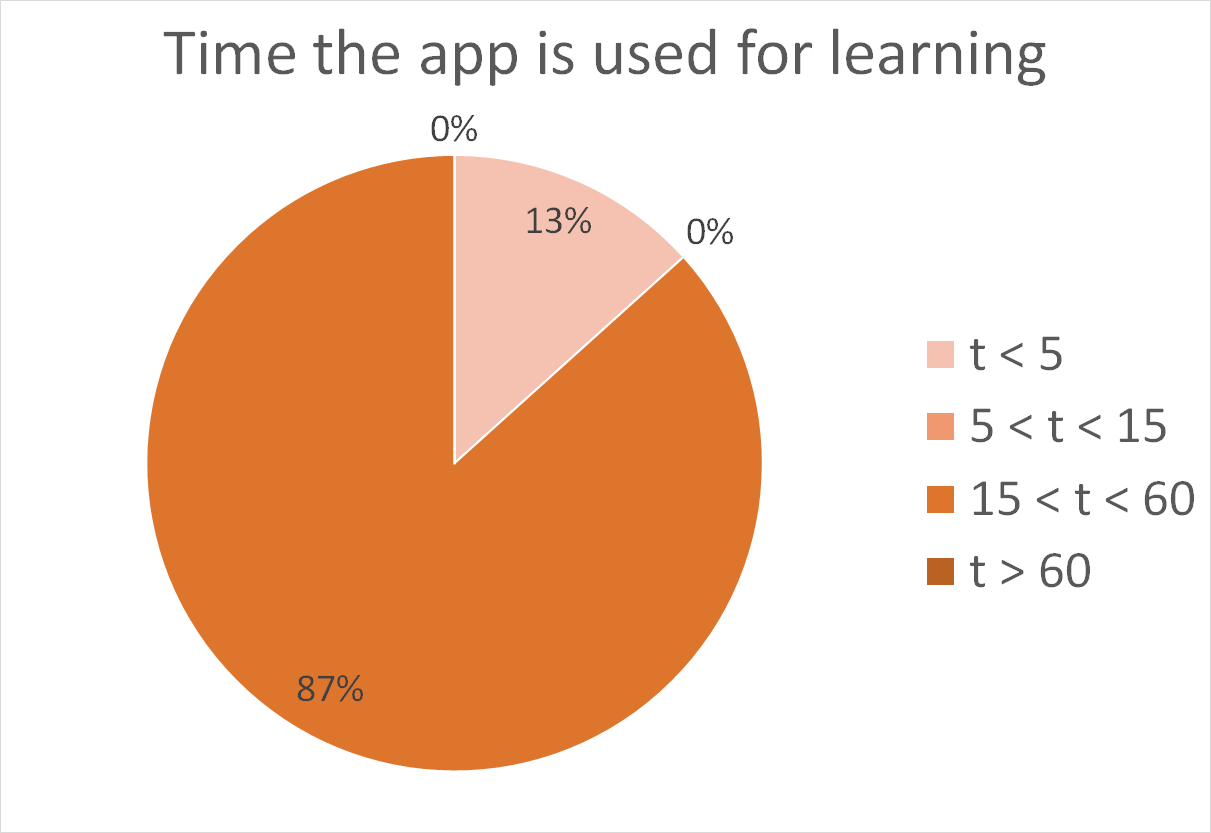
\includegraphics[width=2.6in]{usage_results/3_usage_learning.png} }}%
    \qquad
    \subfloat[Testperson 4]{{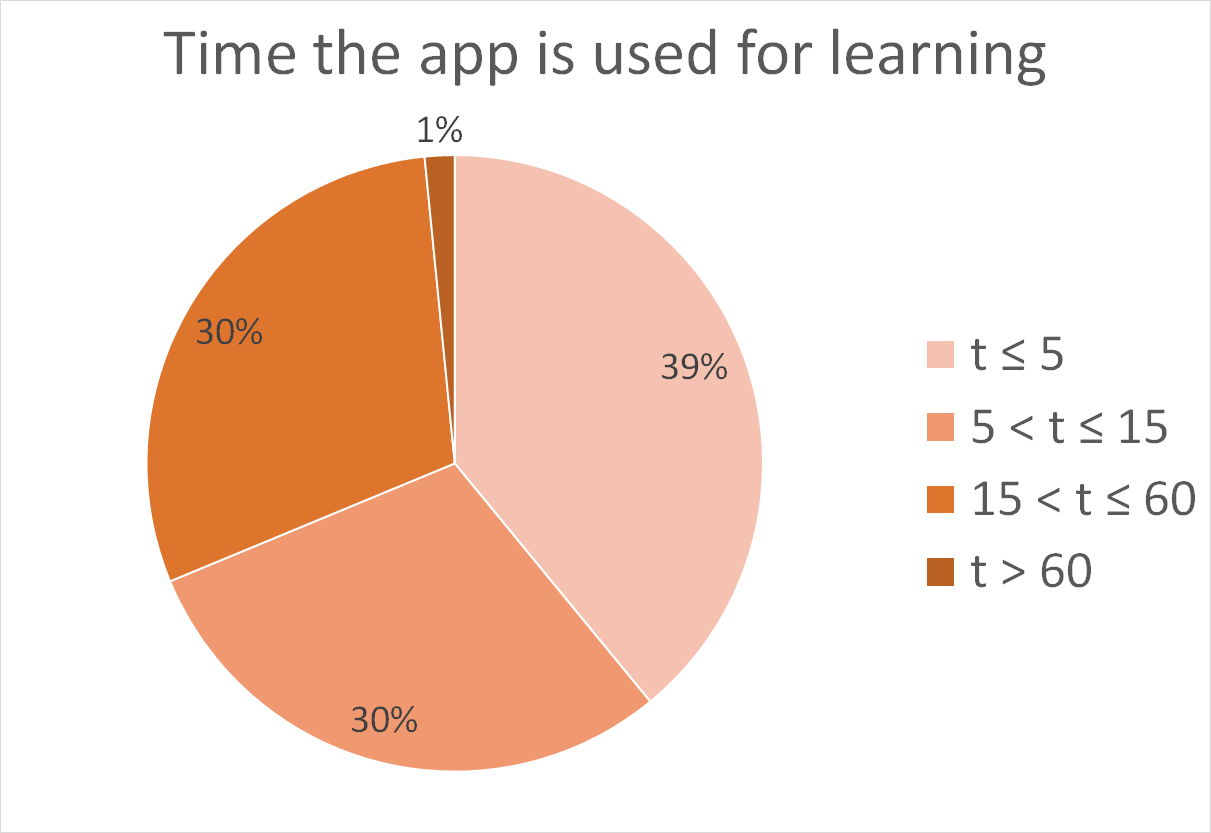
\includegraphics[width=2.6in]{usage_results/4_usage_learning.png} }}%
    \caption{Learning sessions time testpersons 3 and 4}%
    \label{fig:example}%
\end{figure}

\begin{figure}[H]%
    \centering
    \subfloat[Testperson 1]{{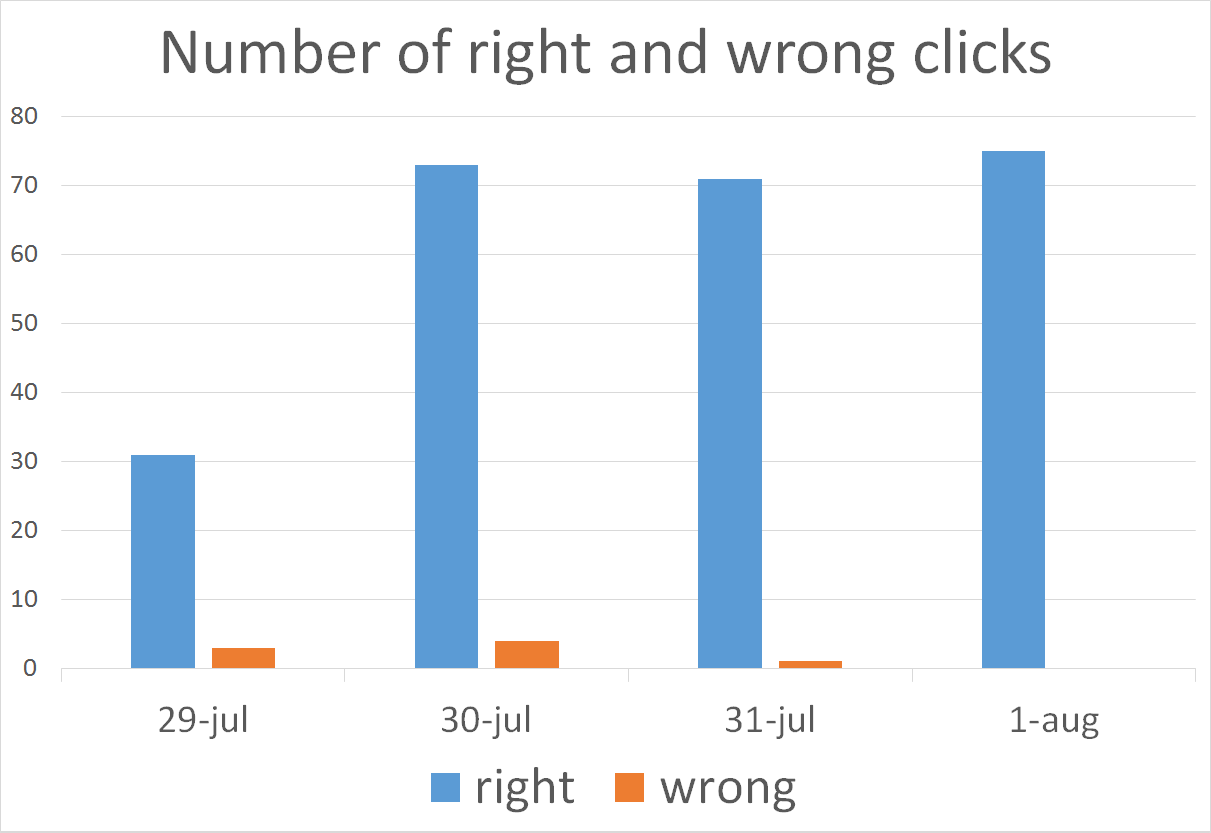
\includegraphics[width=2.6in]{usage_results/1_right_wrong.png} }}%
    \qquad
    \subfloat[Testperson 2]{{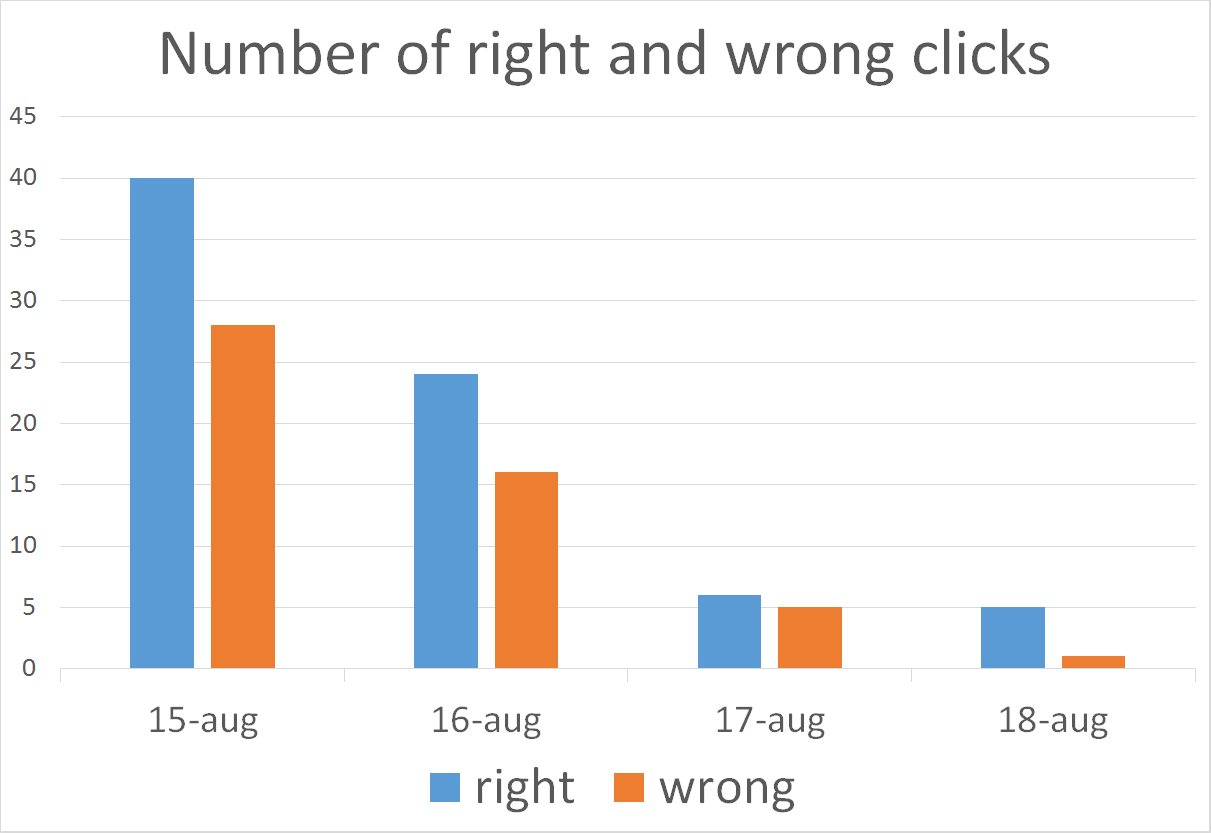
\includegraphics[width=2.6in]{usage_results/2_right_wrong.png} }}%
    \caption{Number of right and wrong clicks for testpersons 1 and 2}%
    \label{fig:example}%
\end{figure}

\begin{figure}[H]%
    \centering
    \subfloat[Testperson 3]{{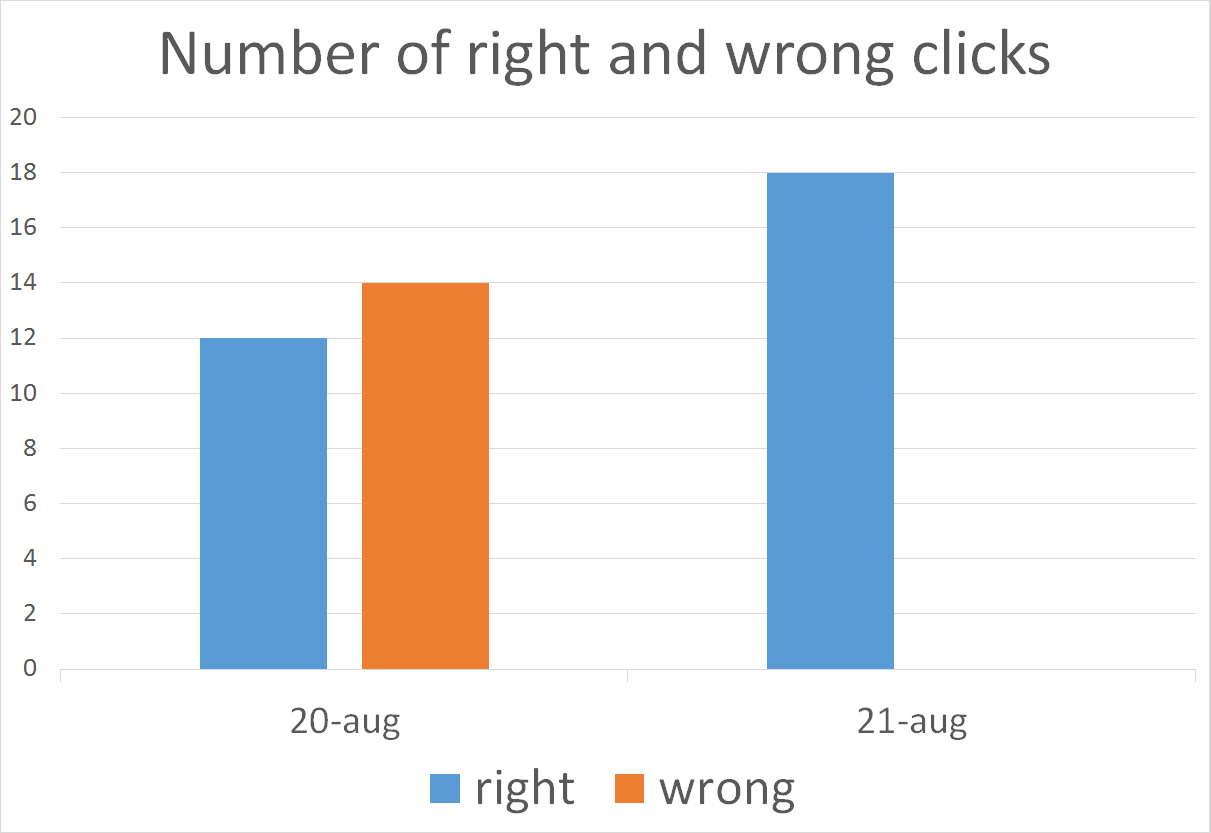
\includegraphics[width=2.6in]{usage_results/3_right_wrong.png} }}%
    \qquad
    \subfloat[Testperson 4]{{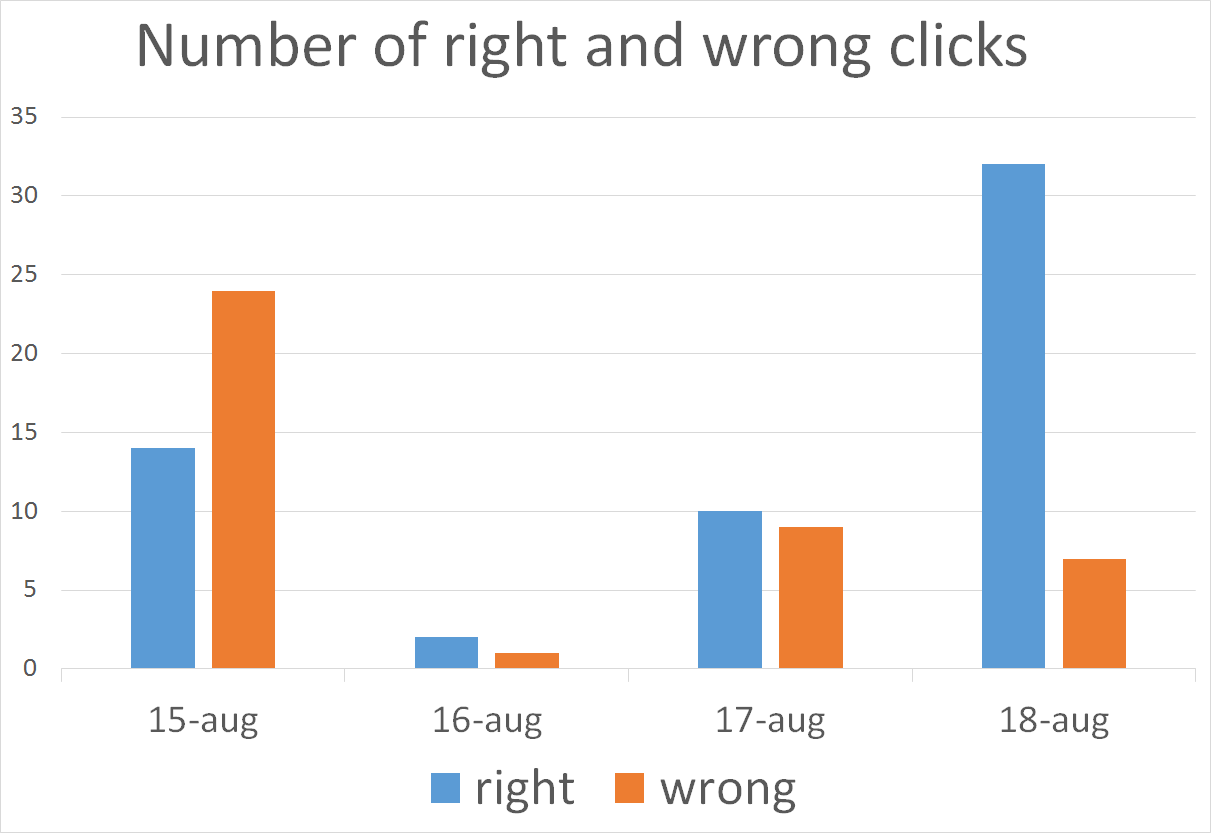
\includegraphics[width=2.6in]{usage_results/4_right_wrong.png} }}%
    \caption{Number of right and wrong clicks for testpersons 3 and 4}%
    \label{fig:example}%
\end{figure}

\begin{table}[H]
\centering
\caption{Testperson 1 average reaction time and total usage time}
\begin{tabular}{| l | l | l |} 
\hline
\textbf{Date} & \textbf{Average} & \textbf{Time} \\ \hline 
29-07-2016 & 00:00:02 & 00:08:39 \\ \hline
30-07-2016 & 00:00:13 & 00:13:10 \\ \hline
31-07-2016 & 00:00:01 & 00:45:43 \\ \hline
01-08-2016 & 00:00:36 & 00:37:07 \\ \hline
\hline
\textbf{Average} & 00:00:07 & 00:26:10 \\ \hline
\textbf{Total} & & 01:44:39 \\ \hline
\end{tabular}
\end{table}

\begin{table}[H]
\centering
\caption{Testperson 2 average reaction time and total usage time}
\begin{tabular}{| l | l | l |} 
\hline
\textbf{Date} & \textbf{Average} & \textbf{Time} \\ \hline 
15-08-2016 & 00:00:08 & 00:19:45 \\ \hline
16-08-2016 & 00:00:02 & 02:15:03 \\ \hline
17-08-2016 & 00:00:02 & 00:36:00 \\ \hline
18-08-2016 & 00:00:02 & 00:01:00 \\ \hline
\hline
\textbf{Average} & 00:00:05 & 00:47:57 \\ \hline
\textbf{Total} & & 02:35:48 \\ \hline
\end{tabular}
\end{table}

\begin{table}[H]
\centering
\caption{Testperson 3 average reaction time and total usage time}
\begin{tabular}{| l | l | l |} 
\hline
\textbf{Date} & \textbf{Average} & \textbf{Time} \\ \hline 
21-08-2016 & 00:04:20 & 00:18:21 \\ \hline
22-08-2016 & 00:00:04 & 00:02:23 \\ \hline
\hline
\textbf{Average} & 00:02:12 & 00:10:22 \\ \hline
\textbf{Total} & & 00:20:44 \\ \hline
\end{tabular}
\end{table}

\begin{table}[H]
\centering
\caption{Testperson 4 average reaction time and total usage time}
\begin{tabular}{| l | l | l |} 
\hline
\textbf{Date} & \textbf{Average} & \textbf{Time} \\ \hline 
16-08-2016 & 00:03:54 & 00:37:23 \\ \hline
17-08-2016 & 00:00:03 & 04:05:46 \\ \hline
18-08-2016 & 00:12:34 & 00:28:02 \\ \hline
19-08-2016 & 00:02:30 & 00:13:41 \\ \hline
\hline
\textbf{Average} & 00:04:45 & 01:21:13 \\ \hline
\textbf{Total} & & 05:24:52 \\ \hline
\end{tabular}
\end{table}

\lstinputlisting[language=JavaScript, caption=script to get different session lengths]{source_code/script_research.js}

\section{Evaluating usage results}
\subsection{General usage}
The graph about the overall usage of the smartwatch tells something about the behavior of the users related to a smartwatch. From the graphs it can be seen that most of the time (53\% till 66\%) the smartwatch is used less than three seconds. This can be related to checking the time what would mean that the ratio between checking the time and learning words is roughly 50 to 50. This is in a well agreement with the design where 50\% of the screen is used for the time and the other 50\% for learning words.\\
The graphs also shows that a session on the smartwatch rarely lasts for more than 60 seconds. Apparently the smartwatch is not suitable or convenient enough to be constantly used for a long period. If the smartwatch is used for a session that lasts a couple of minutes then this will not be longer than fifteen seconds in most cases.

\subsection{Learning sessions}
The graph about the learning sessions shows a different distribution when it comes to the duration of the sessions. When the smartwatch is used to learn words, the session last for 5 till 60 seconds most of the time where the interval of 15 till 60 seconds is often the largest. Sessions that are used for learning and that last for more than 60 seconds are still a small percentage of all the sessions. In the graph from testperson 3 the distribution is a little bit skewed, this is probably due to a lack of results. This user didn't use the watch as often as the other users.

\subsection{Right and wrong}
If we look at all the graphs, it is easily seen that right is more often pressed than wrong. This is something you probably wouldn't expect, since you are learning new words which you don't know. In the graph of testperson 1 this is shown extreme, this user had a german background. This might be a possible explanation for the absurd high number of right clicks. In the graph of testperson 2, a decrease in usage is seen. At 17 augustus the watch it's battery was depleted, so therefore usage was less. At 18 augustus usage was less since it was not an full day of usage, the user handed in the watch at noon. In the graph of testperson 3 it can be seen that the watch is unfortunately only used for 2 days, there is however a clear learning curve which can only be observed in testperson 1 and 4. 

\subsection{Reaction time reveal to right/wrong}
\begin{itemize}
\item Long reaction time; they might want to learn that specific word and be reminded of that again when looking at the time.
\end{itemize}

\chapter {Conclusion and Future Work}
How do users use a smartwatch application to accelerate the memorization process of somebody who is learning the vocabulary of a second language?\\
The users that use a smartwatch application to learn new words mostly use micro learning in order to learn new words. The sessions that last for 5 till 60 seconds occur most of the time. 

\begin{itemize}
\item How long takes a session on a smartwatch (i.e., general usage)? And how long does a learning session take on a smartwatch (i.e., only using time to learn app)?
\item Where is the smartwatch primary for used when using the time to learn app (i.e., for looking at the time or learning words)?
\item How long do they use the app?
\end{itemize}

\begin{appendices}
\chapter{Test Cases}
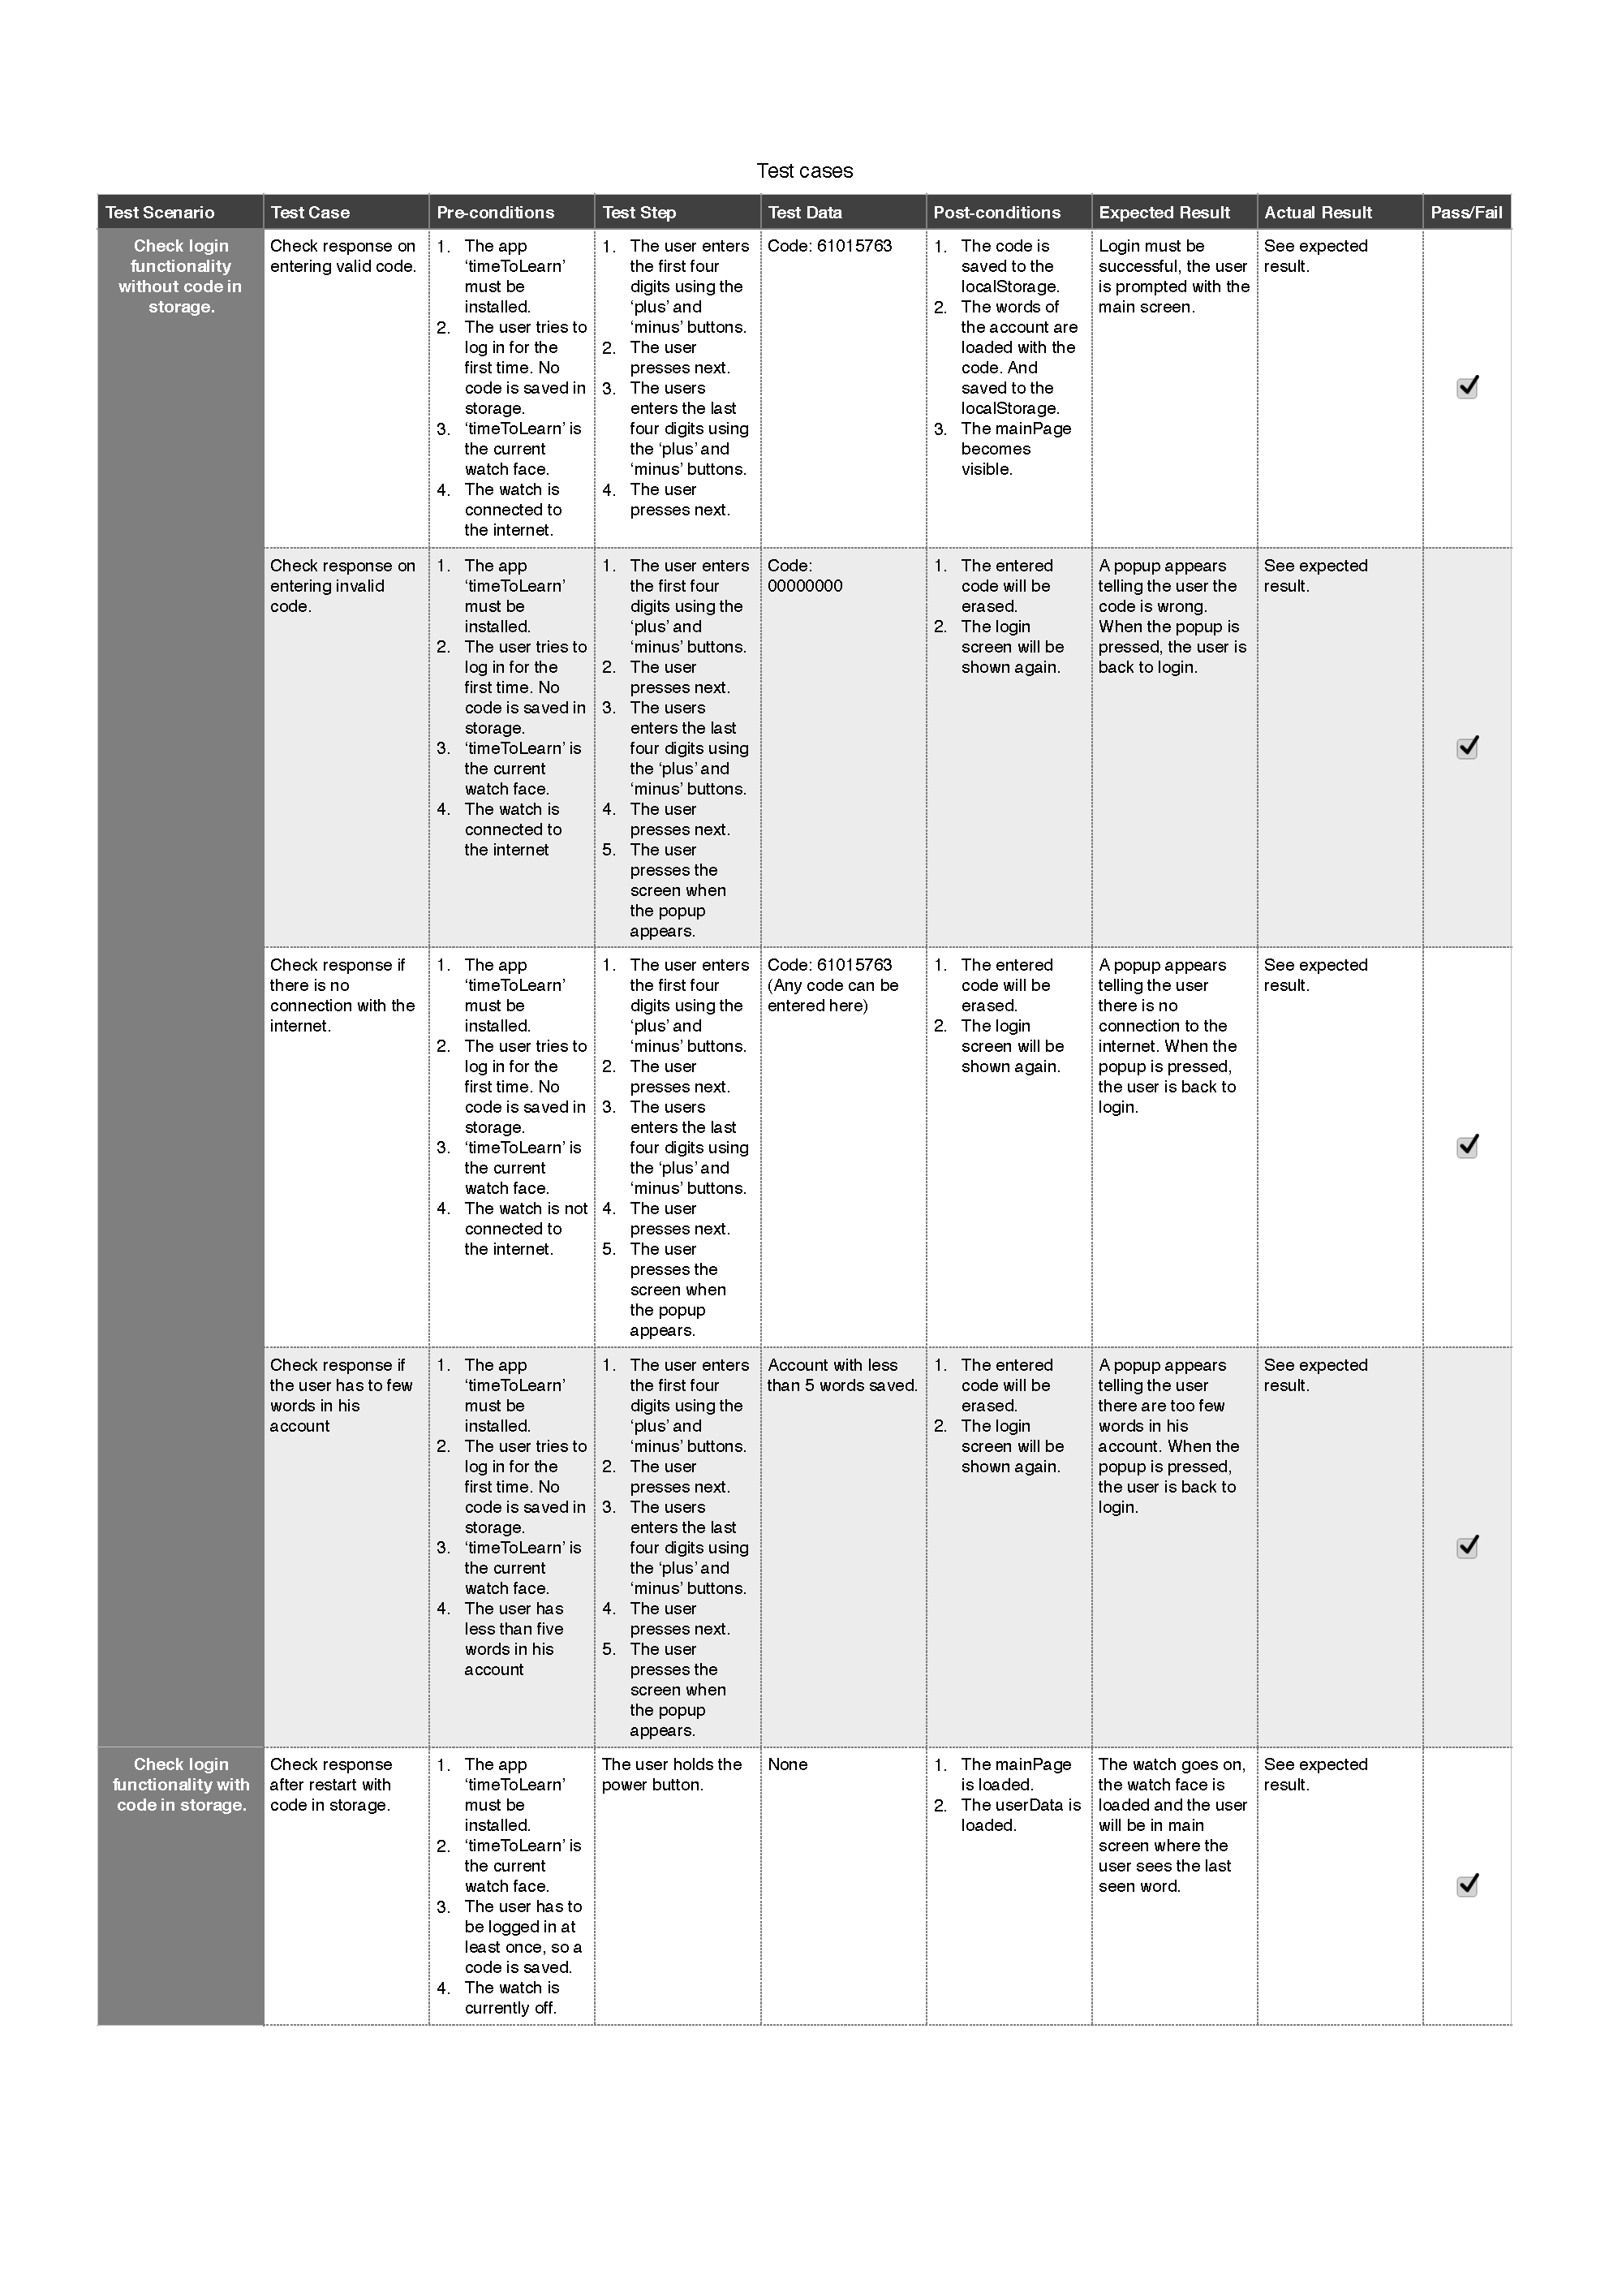
\includepdf[pages=-]{test_cases.pdf}
\chapter{Another one}
\end{appendices}


%END Doc
%-------------------------------------------------------

\bibliography{references}
\bibliographystyle{plain}

\end{document}